% Options for packages loaded elsewhere
\PassOptionsToPackage{unicode}{hyperref}
\PassOptionsToPackage{hyphens}{url}
\PassOptionsToPackage{dvipsnames,svgnames,x11names}{xcolor}
%
\documentclass[
]{article}
\usepackage{amsmath,amssymb}
\usepackage{iftex}
\ifPDFTeX
  \usepackage[T1]{fontenc}
  \usepackage[utf8]{inputenc}
  \usepackage{textcomp} % provide euro and other symbols
\else % if luatex or xetex
  \usepackage{unicode-math} % this also loads fontspec
  \defaultfontfeatures{Scale=MatchLowercase}
  \defaultfontfeatures[\rmfamily]{Ligatures=TeX,Scale=1}
\fi
\usepackage{lmodern}
\ifPDFTeX\else
  % xetex/luatex font selection
\fi
% Use upquote if available, for straight quotes in verbatim environments
\IfFileExists{upquote.sty}{\usepackage{upquote}}{}
\IfFileExists{microtype.sty}{% use microtype if available
  \usepackage[]{microtype}
  \UseMicrotypeSet[protrusion]{basicmath} % disable protrusion for tt fonts
}{}
\makeatletter
\@ifundefined{KOMAClassName}{% if non-KOMA class
  \IfFileExists{parskip.sty}{%
    \usepackage{parskip}
  }{% else
    \setlength{\parindent}{0pt}
    \setlength{\parskip}{6pt plus 2pt minus 1pt}}
}{% if KOMA class
  \KOMAoptions{parskip=half}}
\makeatother
\usepackage{xcolor}
\usepackage[margin=1in]{geometry}
\usepackage{graphicx}
\makeatletter
\def\maxwidth{\ifdim\Gin@nat@width>\linewidth\linewidth\else\Gin@nat@width\fi}
\def\maxheight{\ifdim\Gin@nat@height>\textheight\textheight\else\Gin@nat@height\fi}
\makeatother
% Scale images if necessary, so that they will not overflow the page
% margins by default, and it is still possible to overwrite the defaults
% using explicit options in \includegraphics[width, height, ...]{}
\setkeys{Gin}{width=\maxwidth,height=\maxheight,keepaspectratio}
% Set default figure placement to htbp
\makeatletter
\def\fps@figure{htbp}
\makeatother
\setlength{\emergencystretch}{3em} % prevent overfull lines
\providecommand{\tightlist}{%
  \setlength{\itemsep}{0pt}\setlength{\parskip}{0pt}}
\setcounter{secnumdepth}{5}
% definitions for citeproc citations
\NewDocumentCommand\citeproctext{}{}
\NewDocumentCommand\citeproc{mm}{%
  \begingroup\def\citeproctext{#2}\cite{#1}\endgroup}
\makeatletter
 % allow citations to break across lines
 \let\@cite@ofmt\@firstofone
 % avoid brackets around text for \cite:
 \def\@biblabel#1{}
 \def\@cite#1#2{{#1\if@tempswa , #2\fi}}
\makeatother
\newlength{\cslhangindent}
\setlength{\cslhangindent}{1.5em}
\newlength{\csllabelwidth}
\setlength{\csllabelwidth}{3em}
\newenvironment{CSLReferences}[2] % #1 hanging-indent, #2 entry-spacing
 {\begin{list}{}{%
  \setlength{\itemindent}{0pt}
  \setlength{\leftmargin}{0pt}
  \setlength{\parsep}{0pt}
  % turn on hanging indent if param 1 is 1
  \ifodd #1
   \setlength{\leftmargin}{\cslhangindent}
   \setlength{\itemindent}{-1\cslhangindent}
  \fi
  % set entry spacing
  \setlength{\itemsep}{#2\baselineskip}}}
 {\end{list}}
\usepackage{calc}
\newcommand{\CSLBlock}[1]{\hfill\break\parbox[t]{\linewidth}{\strut\ignorespaces#1\strut}}
\newcommand{\CSLLeftMargin}[1]{\parbox[t]{\csllabelwidth}{\strut#1\strut}}
\newcommand{\CSLRightInline}[1]{\parbox[t]{\linewidth - \csllabelwidth}{\strut#1\strut}}
\newcommand{\CSLIndent}[1]{\hspace{\cslhangindent}#1}
\usepackage[left]{lineno}
\usepackage{ragged2e}
\usepackage{caption}
\usepackage{longtable}
\usepackage[labelformat = empty]{caption}
\usepackage{afterpage}
\usepackage{mdframed}
\usepackage{fontenc}
\usepackage{soul}
\usepackage{xcolor}
\usepackage{float}
\usepackage[symbol]{footmisc}
\definecolor{bleu}{HTML}{2200cc}
\renewcommand{\thefootnote}{\fnsymbol{footnote}}
\usepackage{rotating}
\usepackage{booktabs}
\usepackage{longtable}
\usepackage{array}
\usepackage{multirow}
\usepackage{wrapfig}
\usepackage{float}
\usepackage{colortbl}
\usepackage{pdflscape}
\usepackage{tabu}
\usepackage{threeparttable}
\usepackage{threeparttablex}
\usepackage[normalem]{ulem}
\usepackage{makecell}
\usepackage{xcolor}
\ifLuaTeX
  \usepackage{selnolig}  % disable illegal ligatures
\fi
\usepackage{bookmark}
\IfFileExists{xurl.sty}{\usepackage{xurl}}{} % add URL line breaks if available
\urlstyle{same}
\hypersetup{
  colorlinks=true,
  linkcolor={bleu},
  filecolor={Maroon},
  citecolor={Blue},
  urlcolor={bleu},
  pdfcreator={LaTeX via pandoc}}

\author{}
\date{\vspace{-2.5em}}

\begin{document}

\raggedright
\LARGE

\textbf{Ecological momentary assessment reveals causal effects of music enrichment on infant mood}

\vspace{0.1in}

\justifying
\normalsize

Eun Cho\textsuperscript{1,\(^{\wedge}\),\(\ast\)} , Lidya
Yurdum\textsuperscript{1,2,\(^{\wedge}\),\(\ast\)}, Ekanem
Ebinne\textsuperscript{1}, Courtney B. Hilton\textsuperscript{3},
Estelle Lai\textsuperscript{3}, Mila Bertolo\textsuperscript{1,4,5}, Pip
Brown\textsuperscript{3}, Brooke Milosh\textsuperscript{6}, Haran
Sened\textsuperscript{7}, Diana I. Tamir\textsuperscript{7}, and Samuel
A. Mehr\textsuperscript{1,3,\(\ast\)}

\small

\textsuperscript{1}Child Study Center, Yale University, New Haven, CT
06520, USA.\\
\textsuperscript{2}Department of Psychology, University of Amsterdam,
Amsterdam 1018WT, Netherlands.\\
\textsuperscript{3}School of Psychology, University of Auckland,
Auckland 1010, New Zealand.\\
\textsuperscript{4}Centre for Research in Brain, Language and Music,
McGill University, Montréal, Quebec, Canada.\\
\textsuperscript{5}Integrated Program in Neuroscience, McGill
University, Montréal, Quebec, Canada.\\
\textsuperscript{6}Donald and Barbara Zucker School of Medicine at
Hofstra/Northwell, Hempstead, NY, USA.\\
\textsuperscript{7}Department of Psychology, Princeton University,
Princeton, NJ 08544, USA.

\(^{\wedge}\)These authors contributed equally.

*Corresponding authors. E-mails:
\href{mailto:eun.cho@yale.edu}{\nolinkurl{eun.cho@yale.edu}},
\href{mailto:lidya.yurdum@yale.edu}{\nolinkurl{lidya.yurdum@yale.edu}},
\href{mailto:sam@auckland.ac.nz}{\nolinkurl{sam@auckland.ac.nz}}

\bigskip

\normalsize
\begin{mdframed}[backgroundcolor=gray!20]
Music appears universally in human infancy with self-evident effects on infant psychophysiology: as many parents know intuitively, infants love to be sung to. The long-term effects of parental singing are unknown, however. In an offset-design exploratory 10-week randomized trial ($N = 110$ families of young infants, $M_{age} = 3.67$ months, 53\% female, 73\% White, retention rate = 92\%), we manipulated the frequency of infant-directed singing via a singing intervention. The results, measured by smartphone-based ecological momentary assessment, show that infant-directed singing causes general post-intervention improvements to infant mood, but not to caregiver mood. The findings also show both the feasibility of longitudinal ecological momentary assessment of young infants and the potential of longer-term and higher-intensity singing interventions to improve health in infancy.

\textbf{Keywords:} music, infancy, parenting, infant-directed song, ecological momentary assessment, EMA
\end{mdframed}

\linenumbers
\bigskip

\section{Introduction}\label{introduction}

Decades of research have demonstrated the profound impact of the quality
of early life experiences on lifelong physical and mental health
(\citeproc{ref-Fries2005}{Fries et al., 2005};
\citeproc{ref-Shonkoff2012}{Shonkoff et al., 2012}). Building on Bowlby
(\citeproc{ref-Bowlby1969}{1969})'s work on attachment, evidence from a
wide variety of approaches and across diverse populations shows that
consistent warmth, care, and responsiveness provided by caregivers is a
key feature of healthy caregiving and positive infant-caregiver
relationships (\citeproc{ref-Schore2005}{Schore, 2005};
\citeproc{ref-Stams2002}{Stams et al., 2002}).

For example, infants who experience emotionally available and responsive
parenting have enhanced social and emotional skills
(\citeproc{ref-Feldman1999}{Feldman et al., 1999};
\citeproc{ref-Steele2008}{Steele et al., 2008}), have later advantages
in school (\citeproc{ref-NICHDEarlyChildCareResearchNetwork2006}{NICHD
Early Child Care Research Network, 2006};
\citeproc{ref-PascoFearon2011}{Pasco Fearon \& Belsky, 2011}), and are
more likely to live a healthy life, both physically
(\citeproc{ref-Puig2013}{Puig et al., 2013}) and mentally
(\citeproc{ref-Shaw2005}{Shaw \& Dallos, 2005}). Conversely, when such
nurturing environments are lacking, adverse consequences manifest,
including altered neural circuit maturation (\citeproc{ref-Wen2017}{Wen
et al., 2017}), impaired cognitive development
(\citeproc{ref-Nelson2007}{Nelson et al., 2007}), diminished
social-emotional competence (\citeproc{ref-Davis2004}{Davis et al.,
2004}), and an increased risk of psychiatric symptoms that may persist
through adulthood (\citeproc{ref-Weissman2006}{Weissman et al., 2006}).
While genetic factors shared between parents and infants can partially
explain such effects, they interact with environmental influences in
complex ways; the foundational role of caregiver attention and care in
healthy development remains evident.

Children face very different chances of receiving the benefits of a
caring and nurturing infant-caregiver relationship, however. Factors
related to risk and resilience, such as caregiver characteristics (e.g.,
age, sex, personality, marital status), cultural background, and
socioeconomic circumstances, together mediated by differential access to
resources and opportunities, interact to shape the variability in early
life experiences (\citeproc{ref-Roubinov2017}{Roubinov \& Boyce, 2017}).
Socioeconomic status, for instance, influences the quantity and quality
of speech directed towards infants (\citeproc{ref-Fernald2013}{Fernald
et al., 2013}), shaping the development of the brain language system
(\citeproc{ref-Cheng2023}{Cheng, Roth, et al., 2023}) and subsequent
language and literacy skills (\citeproc{ref-Hemmerechts2017}{Hemmerechts
et al., 2017}). Moreover, contextual factors, such as poor marital
relationship quality (\citeproc{ref-Dennis2006}{Dennis \& Ross, 2006})
and inadequate social support (\citeproc{ref-Reid2015}{Reid \& Taylor,
2015}), are associated with increased risk of postpartum depression,
affecting caregiver responsiveness and sensitivity towards infants
(\citeproc{ref-Feldman2009}{Feldman et al., 2009}).

The high degree of variability in early home environments presents an
opportunity to improve outcomes for young infants and their families. In
particular, simple, low-cost, and low-tech interventions that involve
only modest adjustments to infant care practices hold particular promise
given their ease of uptake. For example, increasing early skin-to-skin
contact (e.g., kangaroo care) has demonstrated numerous health benefits
for both premature and full-term infants worldwide
(\citeproc{ref-Feldman2014}{Feldman et al., 2014};
\citeproc{ref-Moore2012}{Moore et al., 2012}). In this paper, we report
an exploratory randomized trial of a high-potential but relatively
unexplored type of enrichment: singing interventions for caregivers of
young infants.

Caregivers universally sing to their infants in the course of
child-rearing (\citeproc{ref-Mehr2019a}{Mehr et al., 2019};
\citeproc{ref-Singh2023}{Singh \& Mehr, 2023}), throughout infancy
(\citeproc{ref-Yan2021}{Yan et al., 2021}), and regardless of family
socioeconomic status (\citeproc{ref-Mehr2014}{Mehr, 2014};
\citeproc{ref-Custodero2003}{Custodero et al., 2003};
\citeproc{ref-Fancourt2018}{Fancourt \& Perkins, 2018a}). Such
infant-directed singing has robust cross-cultural regularities
(\citeproc{ref-Hilton2022a}{Hilton, Moser, et al., 2022};
\citeproc{ref-Yurdum2023}{Yurdum et al., 2023};
\citeproc{ref-Mehr2019a}{Mehr et al., 2019}), including multimodal
features that combine voice, touch, eye-contact, and movement, which
infants may reciprocate via visual attention, cooing, smiling, and
moving their hands and legs (\citeproc{ref-Malloch2009}{Malloch \&
Trevarthen, 2009}). These interactive behaviours may support a variety
of communicative functions (\citeproc{ref-Trehub2019}{Trehub \&
Gudmundsdottir, 2019}; \citeproc{ref-Mehr2021}{Mehr et al., 2021}),
including signaling social information (\citeproc{ref-Mehr2016}{Mehr et
al., 2016}; \citeproc{ref-Mehr2017b}{Mehr \& Spelke, 2017}) or parental
investment (\citeproc{ref-Kotler2019}{Kotler et al., 2019};
\citeproc{ref-Mehr2017a}{Mehr et al., 2017};
\citeproc{ref-Mehr2017b}{Mehr \& Spelke, 2017}), enhancing social bonds
(\citeproc{ref-Fancourt2018}{Fancourt \& Perkins, 2018a}), and promoting
meaningful social interactions in families
(\citeproc{ref-Lense2022}{Lense et al., 2022};
\citeproc{ref-Malloch1999}{Malloch, 1999}).

It is unsurprising, therefore, that music and infant-directed singing
have profound effects on infants. These have been studied in a variety
of contexts. For example, infant-directed singing captures and sustains
infant attention (\citeproc{ref-Costa-Giomi2014}{Costa-Giomi \& Ilari,
2014}; \citeproc{ref-Nakata2004}{Nakata \& Trehub, 2004};
\citeproc{ref-Trehub2016}{Trehub et al., 2016}) and regulates arousal
and mood (\citeproc{ref-Cirelli2020b}{Cirelli et al., 2020};
\citeproc{ref-Corbeil2016}{Corbeil et al., 2016};
\citeproc{ref-Shenfield2003}{Shenfield et al., 2003}) on a short-term
basis. In some cases, musical stimuli show stronger effects than
infant-directed speech studies: after a still-face procedure,
parent-produced familiar infant-directed songs reduced negative affect
more strongly than infant-directed speech
(\citeproc{ref-Cirelli2020}{Cirelli \& Trehub, 2020}), and in an
open-ended listening task, infants become fussy after approximately
twice as much time when hearing singing, relative to speech
(\citeproc{ref-Corbeil2016}{Corbeil et al., 2016}). Such effects do not
depend fully on the familiarity of the music, however: even unfamiliar,
foreign lullabies calm infants, as measured by heart rate, electrodermal
activity, and pupillometry (\citeproc{ref-Bainbridge2021}{Bainbridge,
Bertolo, et al., 2021}).

Moreover, the effects of infant-directed singing may extend beyond
infants to caregivers themselves. For example, they may aid in the
regulation of caregivers' own arousal levels
(\citeproc{ref-Cirelli2020}{Cirelli \& Trehub, 2020};
\citeproc{ref-Fancourt2018a}{Fancourt \& Perkins, 2018b}); reduce
caregiving-related stress (\citeproc{ref-Cho2021}{Cho \& Ilari, 2021});
or enhance perceived well-being and affective connection with their
infants (\citeproc{ref-Fancourt2017}{Fancourt \& Perkins, 2017};
\citeproc{ref-Steinberg2021}{Steinberg et al., 2021}).

Singing therefore has substantial potential as an enrichment
intervention, as all of the above short-term effects could in principle
work cumulatively, leading to improved health outcomes in infants and
caregivers. Curiously, this idea has largely gone untested, as most
studies of health outcomes related to music in infancy focus on
short-term effects of music interventions in hospital settings (e.g.,
\citeproc{ref-Arnon2014}{Arnon et al., 2014};
\citeproc{ref-Filippa2013}{Filippa et al., 2013}).

Here, we report an exploratory randomized trial of young
infant-caregiver dyads, wherein we experimentally manipulated the
frequency of infant-directed singing via a singing intervention. We
measured outcomes primarily with smartphone-based ecological momentary
assessment (EMA), a method that samples infant behavior naturalistically
via many brief, repeated-measures surveys that caregivers complete daily
at random intervals (e.g., \citeproc{ref-deBarbaro2023}{Barbaro et al.,
2023}; \citeproc{ref-Franchak2019}{Franchak, 2019}).

\clearpage

\begingroup\fontsize{6}{8}\selectfont

\begin{ThreePartTable}
\begin{TableNotes}[para]
\item \textbf{Table 1 | Demographic characteristics of the sample. } 
\item Participants in New Zealand reported their household income in New Zealand dollars, so their responses have been converted to the approximate equivalent US-dollar category. The US-based and New Zealand-based versions of the demographics surveys included slightly different race labels, in line with local guidelines. For simplicity, we have combined the (US-based) category "White" and (New Zealand-based) category "European/New Zealand European".
\end{TableNotes}
\begin{longtable}{llrl}
\toprule
Characteristic &   & n & \% of sample\\
\midrule
 & United States of America & 59 & 54.00\\
\cmidrule{2-4}\nopagebreak
 & New Zealand & 38 & 35.00\\
\cmidrule{2-4}\nopagebreak
 & Canada & 10 & 9.00\\
\cmidrule{2-4}\nopagebreak
 & Singapore & 1 & 1.00\\
\cmidrule{2-4}\nopagebreak
\multirow{-5}{*}{\raggedright\arraybackslash Country of residence} & Sweden & 1 & 1.00\\
\cmidrule{1-4}\pagebreak[0]
 & United States of America & 52 & 48.00\\
\cmidrule{2-4}\nopagebreak
 & New Zealand & 27 & 25.00\\
\cmidrule{2-4}\nopagebreak
 & Canada & 7 & 6.00\\
\cmidrule{2-4}\nopagebreak
 & South Korea & 7 & 6.00\\
\cmidrule{2-4}\nopagebreak
 & United Kingdom of Great Britain and Northern Ireland & 3 & 3.00\\
\cmidrule{2-4}\nopagebreak
 & India & 2 & 2.00\\
\cmidrule{2-4}\nopagebreak
 & Australia & 1 & 1.00\\
\cmidrule{2-4}\nopagebreak
 & China & 1 & 1.00\\
\cmidrule{2-4}\nopagebreak
 & El Salvador & 1 & 1.00\\
\cmidrule{2-4}\nopagebreak
 & France & 1 & 1.00\\
\cmidrule{2-4}\nopagebreak
 & Germany & 1 & 1.00\\
\cmidrule{2-4}\nopagebreak
 & Hong Kong (S.A.R.) & 1 & 1.00\\
\cmidrule{2-4}\nopagebreak
 & Iraq & 1 & 1.00\\
\cmidrule{2-4}\nopagebreak
 & Malaysia & 1 & 1.00\\
\cmidrule{2-4}\nopagebreak
 & Saudi Arabia & 1 & 1.00\\
\cmidrule{2-4}\nopagebreak
 & Spain & 1 & 1.00\\
\cmidrule{2-4}\nopagebreak
\multirow{-17}{*}{\raggedright\arraybackslash Parent's country of birth} & Zimbabwe & 1 & 1.00\\
\cmidrule{1-4}\pagebreak[0]
 & White/European/New Zealand European & 80 & 73.00\\
\cmidrule{2-4}\nopagebreak
 & Asian & 20 & 18.00\\
\cmidrule{2-4}\nopagebreak
 & Black or African American & 2 & 2.00\\
\cmidrule{2-4}\nopagebreak
 & Māori & 1 & 1.00\\
\cmidrule{2-4}\nopagebreak
 & More than one race & 5 & 5.00\\
\cmidrule{2-4}\nopagebreak
\multirow{-6}{*}{\raggedright\arraybackslash Parent race/ethnicity} & I'd prefer not to say & 1 & 1.00\\
\cmidrule{1-4}\pagebreak[0]
 & High school or equivalent & 4 & 4.00\\
\cmidrule{2-4}\nopagebreak
 & Vocational/technical school (2 year) & 2 & 2.00\\
\cmidrule{2-4}\nopagebreak
 & Some college/university & 9 & 8.00\\
\cmidrule{2-4}\nopagebreak
 & College/university graduate & 49 & 45.00\\
\cmidrule{2-4}\nopagebreak
 & Master's degree (MA or equivalent) & 32 & 29.00\\
\cmidrule{2-4}\nopagebreak
 & Doctoral degree (PhD or equivalent) & 4 & 4.00\\
\cmidrule{2-4}\nopagebreak
\multirow{-7}{*}{\raggedright\arraybackslash Parent's highest level of education} & Professional degree (MD, JD, etc) & 9 & 8.00\\
\cmidrule{1-4}\pagebreak[0]
 & Over \$150,000 & 30 & 28.00\\
\cmidrule{2-4}\nopagebreak
 & \$100,000 to \$150,000 & 25 & 23.00\\
\cmidrule{2-4}\nopagebreak
 & \$75,000 to \$99,999 & 26 & 24.00\\
\cmidrule{2-4}\nopagebreak
 & \$50,000 to \$74,999 & 14 & 13.00\\
\cmidrule{2-4}\nopagebreak
 & Below \$50,000 & 9 & 8.00\\
\cmidrule{2-4}\nopagebreak
\multirow{-6}{*}{\raggedright\arraybackslash Current household income (USD)} & I'd prefer not to say & 5 & 5.00\\
\bottomrule
\insertTableNotes
\end{longtable}
\end{ThreePartTable}
\endgroup{}

\section{Methods}\label{methods}

\subsection{Participants}\label{participants}

All participants provided informed consent under a protocol approved by
the Yale University Institutional Review Board (protocol \#2000035858).
We advertised the study via in-person visits to baby fairs, distribution
of flyers at local daycare centers, preschools, and delivery hospitals,
and a public radio advertisement in New Haven, Connecticut. Online
recruitment efforts targeted social media groups for expecting and new
parents, along with online communities related to early childhood
education.

The inclusion criteria required participants to have a smartphone, to
communicate and complete surveys in English, and to be a primary
caregiver of the focal infant. Participants were primarily located in
the United States and New Zealand (see Table 1), but as the study took
place entirely online, there were no geographical constraints. At three
points in the study, caregivers reported their level of involvement in
caregiving on a daily basis. Most caregivers (\emph{n} = 103) reported
providing at least 50\% of childcare at all three time points. Most
participants had some degree of musical training; only 18 out of 110
participants reported having had no formal musical training (see
Supplementary Table 1).

Of the 120 participants initially recruited, two withdrew from the study
due to time constraints. Eight participants were excluded due to low
completion rates, having responded to fewer than 50\% of EMA pings
either for two consecutive weeks during the study period or by the end
of the study (an exclusion criterion determined before data collection
began). This resulted in a final sample size of 109, indicating a
retention rate of 92\%.

We recruited the primary caregivers of infants a maximum of 9 months of
age, but with a focus on younger infants. The participating infants
were, on average, 3.66 months old at the start of the study (range: 0.17
- 8.93 months, interquartile range: 2.13 months; see Supplementary
Figure 1 for a histogram of infant ages). Five infants were born
pre-term (i.e., more than 3 weeks before their due date), and 57 of the
infants were female. Caregivers were predominantly mothers (Mean age:
33.52 years; 103 female, 6 male), and were mostly White, highly
educated, and socioeconomically advantaged (see Table 1 for
demographics).

Participants incentives included digital gift cards, a baby songbook,
and baby clothing (a total value of approximately US\$70), distributed
over the course the study. We also informed caregivers at the outset of
the study that they would receive a personalized report summarizing
their survey responses. This approach, inspired by gamified citizen
science (e.g., \citeproc{ref-Long2023}{Long et al., 2023};
\citeproc{ref-Liu2023}{Liu, Hilton, et al., 2023}), served as an
additional motivation for study completion. An example report is in
Supplementary Figure 2.

\subsection{Study structure}\label{study-structure}

We used an offset-randomised control trial design, with participants
randomly assigned to either a manipulation (\emph{n} = 54) or control
group (\emph{n} = 56). Study participation lasted for 10 weeks, with a
4-week singing intervention period (Figure 1). Assignment was fully
random except for a few participants whose initial random assignment
created an imbalance across the two groups. The manipulation group
received the singing intervention during weeks 2--5 and the control
group received the same intervention following the post-test period
(weeks 7-10). As such, the first 6 weeks of the study comprised a
pre-test, intervention, and post-test period, wherein the only
difference between the groups was whether or not they had received the
singing intervention.

\begin{figure}[H]

{\centering 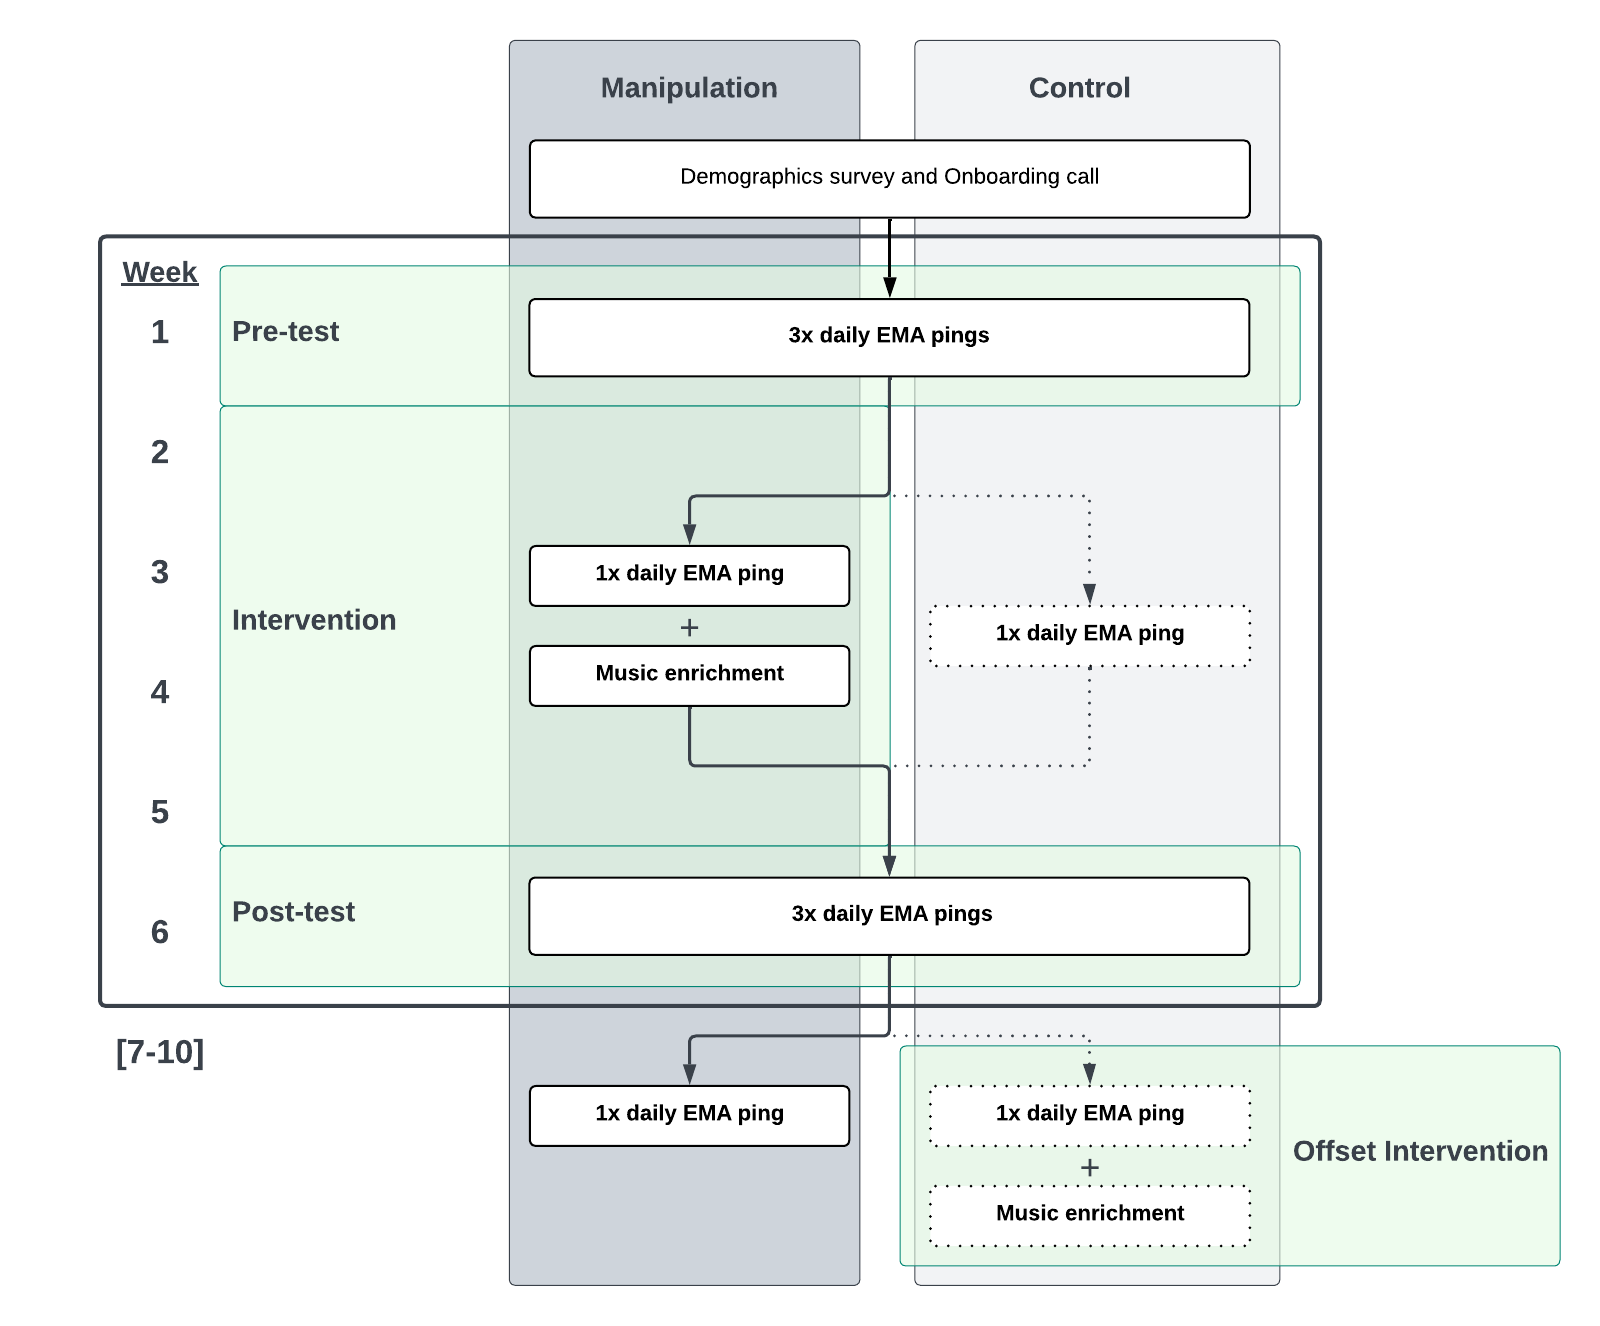
\includegraphics[width=0.9\linewidth,]{../viz/figure1} 

}

\caption{\textbf{Figure 1 | Structure of the experiment.} We conducted an offset-design randomized trial with a one-week pre-test, a four-week intervention, and a one-week post-test (see the areas highlighted in green). This main study period was followed by four further weeks of study participation, to accommodate the offset intervention period (for the control group). The left and right columns indicate the study flow for the manipulation and control groups, respectively. Both groups received the same number of EMA pings and followed identical procedures, except during the intervention period (weeks 2-5), during which the manipulation group participated in the music enrichment intervention along with their daily EMA pings, while the control group only completed the EMA pings and had no intervention.}\label{fig:figure 1}
\end{figure}

Week 1 served as a pre-test, providing baseline EMA data for all
families at high intensity (three pings per day). In Weeks 2-5,
caregivers in the manipulation group underwent the intervention (see
\emph{Singing intervention}), while the control group received no
intervention; during this period, EMA continued at a lower frequency of
one ping per day for all families. Week 6 served as a post-test, with a
high intensity EMA. Caregivers in the control group received the
intervention during Weeks 7-10 while all families having the lower EMA
frequency.

The study began with a one-on-one onboarding video call, where a
designated researcher provided an overview of the study, guided
participants in setting up to receive daily EMA notifications on their
smartphones (see \emph{Measures}), and answered any questions.
Participants were required to be physically present with their infants
during the onboarding session to safeguard against fraudulent
participation, a common concern in online developmental studies (Perkel,
2020). The same researcher continued to serve as the participant's point
of contact throughout the rest of the study.

\subsection{Singing intervention}\label{singing-intervention}

The goal of the intervention was to increase the frequency of
infant-directed singing in daily life while also expanding caregivers'
repertoire of songs. We aimed to do so by teaching participants new
songs to sing at home and providing materials designed to encourage more
singing, in general, in the course of their caregiving.

During the intervention, participants were given access to six
instructional videos of unfamiliar songs presented in karaoke style,
with lyrics synchronized to a bouncing ball indicating the rhythm (all
videos are available at
\url{https://github.com/themusiclab/musical-babies}). These videos were
accessible either via The Person Project app or private YouTube links,
depending on the type of EMA caregivers used (see Supplementary Text 1).
Three videos were sent at the start of the intervention, with an
additional three delivered halfway through. The songs were sourced from
vintage songbooks and online archives of folk songs for children, then
adapted for simplicity and ease of singing, especially for caregivers
with limited music training. This process involved moderate rewriting
and arranging. The songs were then recorded and produced by members of
the research team who had extensive experience in early childhood music
education (authors E.C., E.E., and S.A.M.).

Additionally, participants received an infant-friendly songbook of their
choice from a provided list (i.e., the Ditty Bird Musical Book series,
Cali's Books series), delivered to their homes at the outset of the
intervention. These books featured pressable buttons to activate song
playback, accompanined by vibrant illustrations and lyrics.

Last, to further motivate caregivers to sing more to their infants, we
sent weekly email newsletters to participants in the manipulation group
during the intervention. The newsletters introduced ideas to incorporate
singing into daily caregiving routines; highlighted the significance of
singing in infancy; and presented research findings relevant to the
benefits of musical parenting, in an easy-to-understand format.

To sustain participants' engagement over the four-week intervention, the
research team maintained regular communication with participants via
text messages and/or emails, providing encouragement and promoting
active involvement. Caregivers were not discouraged from singing outside
of the intervention period; the intervention should be understood as
supplementing existing levels of singing in the home, as opposed to
suppressing such behaviors at non-intervention periods or in the control
group.

\subsection{Measures}\label{measures}

The primary measures of infant and caregiver health were collected via
EMA. We used a varied EMA schedule, with caregivers receiving one EMA
survey per day throughout the study, at a random time during waking
hours, except during two high-intensity weeks: Week 1 (pre-test) and
Week 6 (post-test), where they received three EMA surveys a day (at
random times in the morning, afternoon, and evening). In total,
caregivers received 98 EMA surveys across the 10 weeks. EMA data
collection was conducted either via The Person Project, a smartphone app
developed by authors H.S. and D.T; or by Qualtrics surveys distributed
by text message, via Inclivio (\url{https://inclivio.com}). Complete
details about EMA distribution are in Supplementary Text 1.

The EMA surveys addressed various elements of infant and caregiver
health within 2-3 hours of receiving an EMA ping, with 12 items on (1)
\emph{infant mood}, measured by self-assessed valence and arousal; (2)
\emph{infant distress and recovery}, assessed through a pictorial scale
of infant fussiness (\citeproc{ref-Adams2019}{Adams et al., 2019}), and
details on soothing techniques and duration for recovery; (3)
\emph{caregiver mood and stress}, measured by self-assessed valence,
impact, and rationality using the 3D Mind Model approach to mental state
assessment (\citeproc{ref-Thornton2020}{Thornton \& Tamir, 2020}), along
with self-reported levels of caregiving-related stress; and (4)
\emph{musical behavior}, measured by the frequency of caregivers'
engagement with focus behavior (i.e., singing, music listening). Three
additional questions concerning the previous day were also included,
such as the estimated frequency of infant-directed singing, the
frequency of infant night waking, and the duration taken to fall back
asleep. On high-density EMA weeks, these questions were only displayed
in pings arriving before 11:30am (for participants who used The Person
Project) and in the first ping of the day (for participants who used
Inclivio).

We also collected data in four longer-form surveys spread throughout the
study, for analysis in a different paper comparing EMA responses to
retrospective surveys; they are not reported here. The full text of the
EMA surveys is in Supplementary Text 2.

\subsection{Compliance}\label{compliance}

On average, participants completed 72.44 of the 98 EMA surveys, for an
overall response rate of 74\%, with a higher rate during the low
intensity weeks (1 EMA survey/day; 78.39\%) than the high intensity
weeks (3 EMA surveys/day; 68\%). This compliance rate is comparable to
those reported in other infant EMA studies, including one-week studies
with intensive daily pings (\citeproc{ref-deBarbaro2023}{Barbaro et al.,
2023}; \citeproc{ref-Wenze2023}{Wenze et al., 2023};
\citeproc{ref-Franchak2019}{Franchak, 2019}) and longitudinal studies
lasting up to 16 weeks with less intensive pings
(\citeproc{ref-Allen2018}{Allen et al., 2018};
\citeproc{ref-Franchak2024}{Franchak et al., 2024};
\citeproc{ref-Corpuz2023}{Corpuz et al., 2023}). Participants' response
rates were unrelated to infant age at the start of the study (\(\beta\)
= 0.00017; \emph{p} = 0.48). The proportion of unanswered pings was
slightly higher in the control group, although this difference did not
reach significance at pre-test (\emph{p} = 0.27), intervention (\emph{p}
= 0.09), or post-test (\emph{p} = 0.06). Given the comparable levels of
missingness in the two groups, we assume that nonresponse represents
missing data at random and did not attempt to account for missingness in
our analyses.

To assess responsiveness to EMA pings, we calculated response latency by
subtracting the time of EMA notification from the time participants
opened the survey on their smartphone. The median response latency was
20.48 mins minutes (high intensity weeks = 16.31 mins; low intensity
weeks = 23.25 mins); this analysis was only available for participants
whose pings were distributed by text message. Latency increased with
infant age (\(\beta\) = 0.09, \emph{SE} = 0.04, \emph{p} = 0.02).

\section{Results}\label{results}

\subsection{Music enrichment increases the frequency of infant-directed
singing}\label{music-enrichment-increases-the-frequency-of-infant-directed-singing}

We began by asking whether the intervention worked; namely, whether we
succeeded in increasing the frequency of infant-directed singing in the
intervention group, relative to the control group. Two EMA items
addressed this question, in different ways.

First, every EMA ping included an item asking caregivers whether they
had sung to their infant in the preceding 2-3 hours (they could respond
``Yes'' or ``No''). Only caregivers who reported having been with their
infants in the last 2-3 hours responded. We dropped data where the
caregiver indicated in the same EMA ping that their infant was sick. In
all analyses comparing the behaviour of the intervention and control
groups within a specific week, we use weekly scores that are calculated
as averages of all responses to EMA pings during that week.

The intervention caused a clear increase in the frequency of
infant-directed song (Figure 2, left panel), with no difference between
groups at pre-test (proportion of ``Yes'' responses in manipulation
group: M = 64\%, SD = 24; in control group: M = 65\%, SD = 22; t(103.69)
= -0.08, \emph{p} = 0.93, two-sample t-test), and a significant
difference at post-test (proportion of ``Yes'' responses in manipulation
group: M = 77\%, SD = 20; in control group: M = 64\%, SD = 24; t(98.88)
= 3.11, \emph{p} = 0.002, difference = 14, two-sample t-test). Note that
during post-test, caregivers were no longer actively being encouraged to
sing more to their infants: week 5 was the last week of the
intervention. The significant difference between groups held despite
this. A mixed-effects time-series model that accounted for
autoregression across the 6 weeks of the study showed a significant
interaction across group and time (\(\beta\) = 0.26, \emph{SE} = 0.12,
\emph{p} = 0.02). In the manipulation group, each week of the
intervention was associated with a 1.85 point increase in the proportion
of times caregivers reported singing to their infants.

\begin{figure}[H]
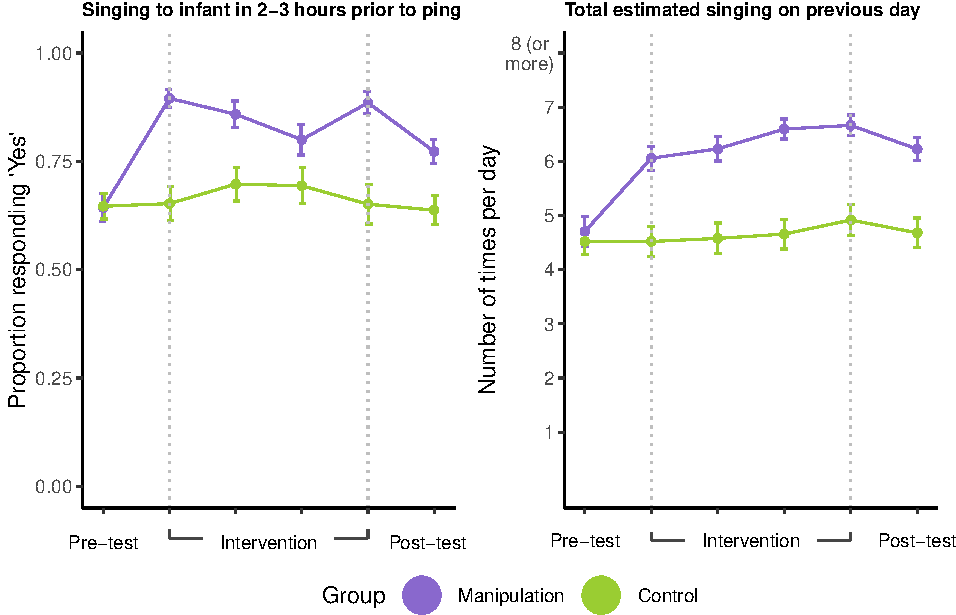
\includegraphics{MIPH_childdev_files/figure-latex/fig2-1} \caption{\textbf{Figure 2 | Music enrichment increases the frequency of infant-directed singing.} The plots depict responses to two items: "Did you sing to [baby] in the last 2-3 hours?" (left panel), asked up to three times per day with response options "Yes" or "No"; and "If you had to guess, how many times did you sing to [baby] yesterday?" (right panel), asked in the first notification of the day (delivered during morning hours between 9 and 11:30 am) with response options ranging from "1" to "8 or more times". There was a sharp increase in infant-directed singing for the manipulation group, but not the control group, as measured by both items; the increase persisted through the full intervention and was maintained in the post-test week. Tick marks indicate the study week; week 1 and 6 correspond to pre- and post-test, respectively, while weeks 2 through 5 span the intervention period. Points denote weekly averages, error bars indicate standard error of the mean.}\label{fig:fig2}
\end{figure}

These effects were specific to infant-directed singing, as we did not
find comparable interaction effects for other music-related variables
that were also reported in the same EMA surveys, such as playing
recorded music for the infant (\(\beta\) = -0.16, \emph{SE} = 0.12,
\emph{p} = 0.18); or caregivers' personal music listening (\(\beta\) =
0.00, \emph{SE} = 0.12, \emph{p} = 0.98) in the 2-3 hours preceding the
EMA ping.

Notably, the absolute frequency of infant-directed singing was
substantial in the manipulation group: by the final week of the
intervention, 89\% of the time, a caregiver had recently sung to their
infant when they received an EMA ping (relative to 65\% in the control
group).

Second, morning EMA pings (i.e., those delivered before 11:30am)
prompted caregivers to report how many times they had sung to their
infant \emph{on the previous day} (``If you had to guess, how many times
did you sing to {[}baby{]} yesterday?'') on an 8-point scale ranging
from ``1'' to ``8 or more times''. Here too we found a clear effect of
the intervention (Figure 2, right panel), with no group-level difference
at pre-test (t(105.29) = 0.51, \emph{p} = 0.61, two-sample t-test), a
significant difference at post-test (t(101.22) = 4.45, \emph{p}
\textless{} .0001, two-sample t-test), and a significant
group-by-timepoint interaction (\(\beta\) = 0.03, \emph{SE} = 0.01,
\emph{p} \textless{} .0001) indicating an average of 0.28 more songs per
week in the manipulation group (roughly 3\% of the scale). While
caregiver reports summarizing the previous day's singing with an integer
may not be optimally precise, at the post-test period these effects
represented a 1.48 unit increase in absolute daily estimates of singing
behaviour (\emph{SD} = 2.19).

Thus, convergent evidence demonstrates that the intervention succeeded
at its primary goal, namely, to experimentally manipulate caregivers'
infant-directed singing in daily life.

\begin{figure}[H]

{\centering 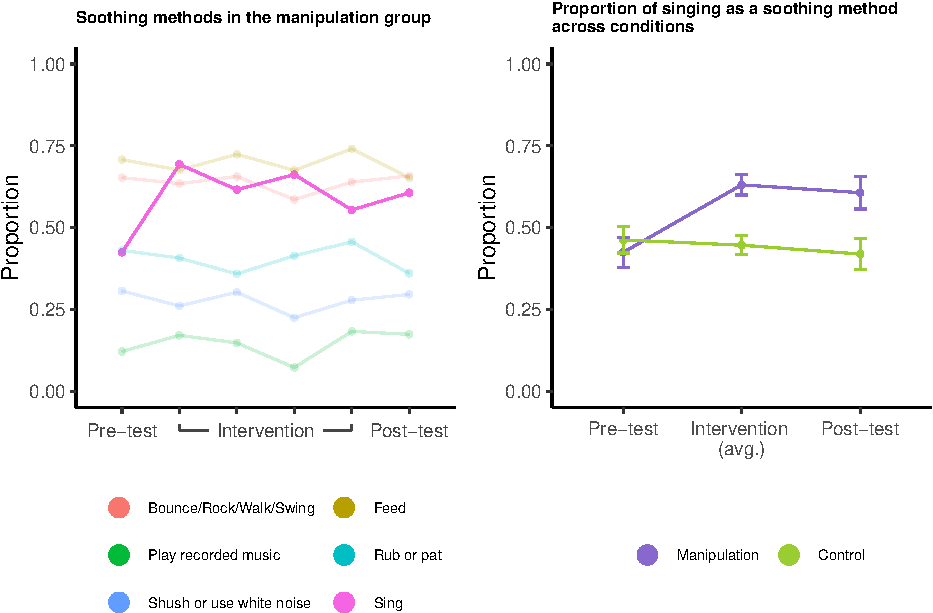
\includegraphics{MIPH_childdev_files/figure-latex/figure-3AB-1} 

}

\caption{\textbf{Figure 3 | Music enrichment alters parent responses to infant fussiness.} In each EMA ping, we asked the parent if their infant was fussy in the previous 2-3 hours; if they answered 'Yes', then we asked how they attempted to soothe the infant. The left panel illustrates the proportion of responses in the manipulation group for six soothing techniques (of 12 available options; see Supplementary Text 2). Tick marks indicate the study week; week 1 and 6 correspond to pre- and post-test, respectively, whereas weeks 2 through 5 span the intervention period. Singing in response to fussiness was the only soothing technique out of 12 that showed an increase in usage from pre- to post-test. This increase was specific to the manipulation group, as shown in the right panel, which rescales the data as a proportion of all responses and averages across the four intervention weeks (weeks 2-5) for simplicity. In the manipulation group, parents used singing in response to fussiness more than half of the time. The points indicate mean scores across the given week(s) and error bars denote standard errors of the mean.}\label{fig:figure-3AB}
\end{figure}

\subsection{Music enrichment increases the use of singing specifically
in the context of soothing
infants}\label{music-enrichment-increases-the-use-of-singing-specifically-in-the-context-of-soothing-infants}

Given the well-known role of music in soothing or calming infants (e.g.,
\citeproc{ref-Bainbridge2021}{Bainbridge, Bertolo, et al., 2021}), we
wondered whether the singing intervention had not only general effects
on the use of infant-directed singing, but also specific effects,
increasing its use in soothing contexts.

It did. In each EMA survey, we asked participants if their infant was
fussy in the last 2-3 hours. If so, they indicated all soothing
techniques they used in response, from a list of 12 different techniques
(e.g., feeding, changing a diaper, shushing, playing recorded music,
singing; the full list is in Supplementary Text 2).

While the use of non-musical soothing techniques remained more-or-less
constant over the course of the study, in the manipulation group there
was a large increase in the proportion of time caregivers used singing
in response to fussy infants (Figure 3, left panel; pre-test: M = 0.44,
SD = 0.31; average across intervention: M = 0.53, SD = 0.41; post-test:
M = 0.51, SD = 0.35). While singing was the third most frequently used
soothing technique among the 12 different techniques (both at pre-test
and overall), following picking-up/bouncing/rocking/swinging and
feeding, singing was the only technique with increased caregiver use as
a result of the intervention, an increase of 18 percentage points from
pre-test to post-test (t(98.72) = 2.71, \emph{p} = 0.008).

No such increase was observed in the control group, however, where the
singing response stayed comparably flat (t(96.97) = -0.70, \emph{p} =
0.49; Figure 3, right panel). The cross-group difference at post-test
was statistically significant (t(97.78) = 2.74, \emph{p} = 0.007).
Notably, we did not observe a group-level difference at post-test in the
frequency of playing recorded music to infants, indicating that the
effect wasn't a general increase in the use of music to soothe infants
(t(88.07) = 0.94, \emph{p} = 0.35).

Thus, the singing intervention not only increased the overall use of
infant-directed singing in daily life, but specifically changed how
caregivers responded to infant fussiness. We note here that no part of
the intervention specifically instructed caregivers to use music in the
context of soothing; the decision to use music in the context of
soothing infants is apparently an intuitive one.

\subsection{Infant-directed singing improves infant mood but not
caregiver
mood}\label{infant-directed-singing-improves-infant-mood-but-not-caregiver-mood}

As music has been shown to affect a variety of affect- and
arousal-related variables in infants, in the short-term (e.g.,
\citeproc{ref-Bainbridge2021}{Bainbridge, Bertolo, et al., 2021};
\citeproc{ref-Cirelli2020}{Cirelli \& Trehub, 2020};
\citeproc{ref-Cirelli2019}{Cirelli et al., 2019};
\citeproc{ref-Corbeil2016}{Corbeil et al., 2016}), a key question for
this randomized trial is whether such effects are cumulative. Does music
enrichment produce lasting effects on infant affect?

To study this question, we focused primarily on caregiver evaluations of
infant mood, reported using a sliding scale from Negative (0) to
Positive (100). In each EMA survey, caregivers rated their infant's mood
during the last 2-3 hours. Caregivers only responded if they had been
with their infant during that time. Importantly, this item does
\emph{not} measure caregivers' perceptions of infants' mood in response
to singing. Rather, the item measures perceptions of infant mood
\emph{in general}.

To account for participant variability in scale usage, we
\emph{z}-scored mood ratings within participants. We then computed a
weekly average score for each infant. Consistent with prior results
showing improvements in mood as infants grow older
(\citeproc{ref-Barr1990}{Barr, 1990}), all infants, on average, showed
improvements in mood from pre- to post-test (mean difference = 0.25,
\emph{t}(102.00) = 4.99, \emph{p} \textless{} .0001). These improvements
were moderated by manipulation group, however (Figure 4, left panel).

At pre-test the two groups did not differ (manipulation group: M =
-0.10, SD = 0.41; control group: M = -0.11, SD = 0.30, \emph{t}(95.76) =
0.18, \emph{p} = 0.86), but at post-test, the singing intervention had
caused a significant difference in infant mood, with the manipulation
group approximately 0.34 standard deviations higher (manipulation group:
M = 0.24, SD = 0.32; control group: M = 0.06, SD = 0.32;
\emph{t}(102.78) = 2.94, \emph{p} = 0.002, one-sided \emph{t}-test).

A mixed-effects time-series model (using untransformed data) that
accounted for autoregression showed a significant interaction term
across group and time (\(\beta\) = 0.18, \emph{SE} = 0.05, \textless{}
.001). In the manipulation group, each week of intervention was
associated with a 1.56 unit increase in the 100-point mood scale for
infants in the manipulation group (\emph{p} \textless{} .001), or
roughly one tenth of a SD increase per week of intervention.

Last, given the exploratory nature of these analyses, we tested whether
the main mood result repeated across both subsets of the main sample: a
first cohort, recruited mainly in the United States from February to
June 2023; and a second cohort, recruited mainly in New Zealand from
June to December 2023. Mixed-effects time-series models revealed the
same expected group-by-time interaction in both the first (\(\beta\) =
0.12, \emph{SE} = 0.06, = 0.04) and second cohorts (\(\beta\) = 0.32,
\emph{SE} = 0.10, = 0.001), although not every subtest replicated (e.g.,
the difference in mood scores at post-test was statistically significant
in the first cohort, \emph{t}(54.20) = 2.49, \emph{p} = 0.008, one-sided
\emph{t}-test; but did not reach significance in the second cohort,
\emph{t}(15.05) = 1.31, \emph{p} = 0.1, one-sided \emph{t}-test. The
significant group-by-time interactions indicate a successful internal
replication, but the smaller effect size in the second cohort suggests a
need for replication.

\begin{figure}[H]
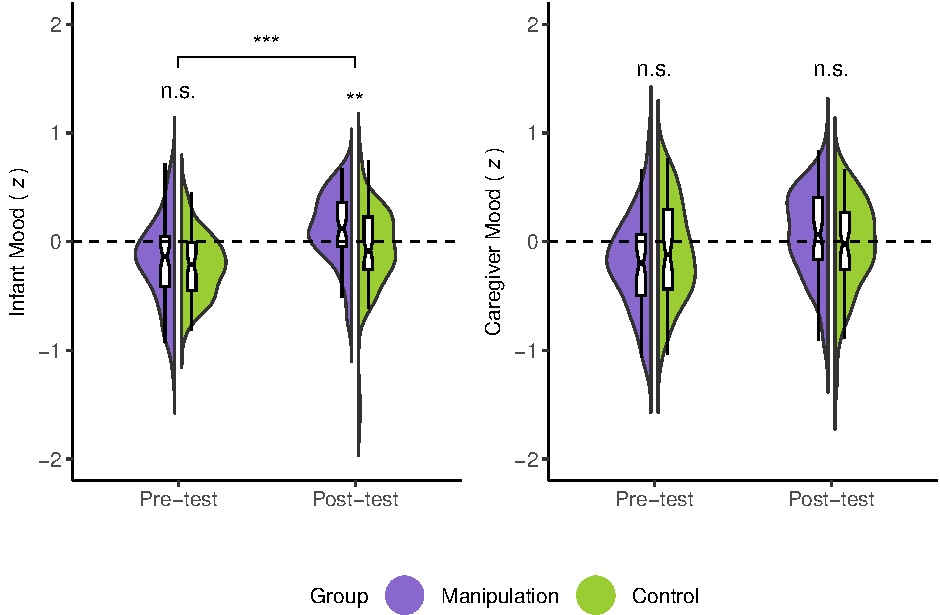
\includegraphics{MIPH_childdev_files/figure-latex/fig4-1} \caption{\textbf{Figure 4 | Music enrichment improves infant mood but not caregiver mood.} In each EMA ping, caregivers were asked to report their infant's mood and their own mood at the moment they received the ping, both on a 100-point slider (anchored at "Very negative" and "Very positive"). We normalized responses within participants to account for individual differences in scale use. While average mood of infants in the two groups did not differ at pre-test, it did at post-test, with significantly more positive mood reports in the manipulation group (left panel). We did not observe the same pattern for caregiver mood (right panel). The half-violins depict the distributions of weekly mean mood ratings from each of the two groups, weighted by participant. The shaded area in the half-violins represent kernel density estimates; the vertical boxplots denote the median (horizontal line), 95\% confidence interval (notches), and interquartile range (edges of the boxes). The significance stars above the violins denote the between-groups comparison at a given time point. The horizontal bar denotes the significant group-by-time interaction in the time-series model. $^{\ast}p < 0.05$, $^{\ast\ast}p < 0.01$, $^{\ast\ast\ast}p < 0.001$.}\label{fig:fig4}
\end{figure}

Caregivers also rated how energetic their infants were in the previous
2-3 hours, using a comparable scale to the mood item; we found no
comparable effects on this measure, suggesting the effects of the
singing intervention are specific to infant mood and do not generalize
to infant arousal.

We proceeded by analyzing data concerning caregiver mood, for two
reasons. First, improvements to infant mood might well translate to
improvements in caregiver mood, since happier infants are easier to look
after than fussier ones. Second, a potential concern with the infant
mood result is the potential for contamination in caregiver
self-reports: they might erroneously report happier infants when they
themselves felt happier; because this trial relies on caregiver EMA
data, we are unable to directly assess infant mood in isolation from the
caregiver.

We addressed these issues with several analyses of caregivers' responses
to ratings of their own mood, completed in the same EMA surveys and
using the same (z-transformed) scale as the infant mood item. In
contrast to infant mood, we found no differences between groups at
pre-test (manipulation group: M = -0.15, SD = 0.46; control group: M =
-0.02, SD = 0.48, \emph{t}(104.90) = -1.42, \emph{p} = 0.16) or
post-test (manipulation group: M = 0.14, SD = 0.43; control group: M =
0.03, SD = 0.48, \emph{t}(101.71) = 1.21, \emph{p} = 0.12). This absence
of effect suggests that the effect of music enrichment on caregiver
self-reports of infant mood does not erroneously represent an effect on
caregiver mood.

Infant mood and caregiver mood were moderately and positively
correlated, however (Spearman's rank correlation; \emph{r} = 0.39,
\emph{p} \textless{} .0001); adding caregiver mood as a predictor to the
mixed model regressing condition and day number on infant mood weakened
the time-by-group interaction enough that it no longer reached
statistical significance (\emph{p} = 0.09). We found no evidence for a
difference in correlation across the manipulation and control groups
(\(\beta\) = 0.01, \emph{p} = 0.59), indicating that any potential
reporting biases were not due to the intervention.

To further assess the degree of potential confounding between infant and
caregiver mood reports, we tested whether each of the infant and
caregiver mood self-reports correlated with third measures that we
expected to be more strongly linked to caregiver mood than infant mood.
Two variables in the daily EMA surveys met this criterion: a measure of
how socially connected caregivers felt (from ``Very lonely'' to ``Very
connected'') and a measure of the perceived stress of caregiving (``How
stressful have you found parenting in the last 2-3 hours?''). Both items
should, in principle, be more strongly associated with caregiver mood
than infant mood, assuming the two mood items are indeed measuring
different real-world constructs.

They were. The association of social connection and caregiver mood
(\(\beta\) = 0.44, \emph{p} \textless{} .0001) was both stronger and in
the opposite direction of the association between social connection and
infant mood (\(\beta\) = -0.08, \emph{p} = 0.02; interaction: \(\beta\)
= 0.002, \emph{p} \textless{} .0001, autoregressive time series model
with untransformed mood data). Similarly, while both infant (\(\beta\) =
-0.02, \emph{p} \textless{} .0001) and caregiver mood (\(\beta\) =
-0.02, \emph{p} \textless{} .0001) predicted how stressful caregivers
found parenting, the interaction between the two mood variables was
statistically significant (\(\beta\) = 0.0001, \emph{p} \textless{}
.0001). These results suggest that our measures of infant mood and
caregiver mood tapped into substantively different mood phenomena in the
study population.

In sum, we found a causal effect of the singing intervention on infant
mood, but not caregiver mood, despite the two mood measures being
correlated with one another. It is possible that increasing the
frequency of infant-directed singing may improve \emph{both} infants'
and caregivers' moods, whether directly (e.g., singing makes caregivers
feel positive) or indirectly (e.g., having a happier infant makes
caregivers feel positive). If so, putative effects on caregiver mood are
small enough that they could not be reliably detected in this brief
intervention study.

\section{Discussion}\label{discussion}

We report evidence that a brief singing intervention increases the
frequency of infant-directed singing, that caregivers intuitively extend
this musical behavior specifically to the context of soothing their
infants, and that these changes in the home musical environment cause
improvements to infant mood in general. This suggests that the immediate
effects of music on infants (e.g.,
\citeproc{ref-Bainbridge2021}{Bainbridge, Bertolo, et al., 2021};
\citeproc{ref-Cirelli2019}{Cirelli et al., 2019}) may be cumulative,
leading to longer-term effects on infants.

Importantly, the main effect of the singing intervention on infant mood
was found in EMA pings that occurred \emph{regardless of whether the
caregiver had recently sung to the infant} (i.e., as opposed to items
asking about infants' mood responses to singing in particular). This
implies that infant-directed singing improved infant mood \emph{in
general}, in a one-week post-test period that followed the intervention
(at which time caregivers were no longer explicitly instructed to sing
to their infants). The present findings therefore substantiate a causal
relationship between an enriched musical environment and general
improvements in infant mood.

Moreover, while this result is supported only by caregiver-observational
data, several considerations suggest that the findings reflect robust
changes in infant affect. First, the data were collected with ecological
momentary assessment, instead of retrospective surveys, and therefore
are unlikely to be contaminated by recall bias
(\citeproc{ref-Stone2002}{Stone \& Shiffman, 2002};
\citeproc{ref-Reis2012}{Reis, 2012}). Second, the results largely
replicated internally, in two separate samples recruited in two
different countries, and therefore are unlikely to reflect the
caregiving practices of only one community. Third, we found no
corresponding effect of the intervention on caregiver mood, suggesting
that caregivers' self-reports of infant mood did not simply reflect
caregivers' own mood, as they might in the presence of a reporting bias
(see Results). Fourth, the modest correlation between caregiver reports
of infant mood and their own mood was of a comparable size in both the
manipulation and control groups, suggesting that an expectancy effect
(e.g., where only parents who had experienced the music intervention
reported erroneously high infant or caregiver mood) did not account for
the main effects. Future studies can further support the veracity of
infant mood assessment via EMA by supplementing the method with direct
lab-based or home-based observations of infant mood and behavior,
psychophysiological measures of infant arousal, and so on.

Infant mood is an important issue for caregivers as it is closely linked
to parenting stress (\citeproc{ref-Oddi2013}{Oddi et al., 2013}),
caregiver-infant bonding and attachment (\citeproc{ref-Nolvi2016}{Nolvi
et al., 2016}; \citeproc{ref-Takacs2020}{Takács et al., 2020}), and
subsequently the infants' social and emotional development
(\citeproc{ref-Steele2008}{Steele et al., 2008};
\citeproc{ref-Shaw2005}{Shaw \& Dallos, 2005}). Such associations raise
the possibility that general improvements in infant mood, caused by
altering the home music environment in young families, could
subsequently cause other positive health-related outcomes. While we did
not observe any such effects here (such as an improvement in caregiver
mood), we note that this study had only a brief (4-week), low-intensity,
self-directed intervention. A longer-term, higher-intensity
intervention, perhaps with direct music instruction from a qualified
teacher, may well uncover more widespread effects. These could
potentially generalize to other health domains that are tightly related
to caregivers' well-being, such as the frequency of infant night waking,
the duration of crying bouts, the ease with which caregivers can calm
their infants when upset, or levels of caregiver stress.

Infant-directed singing is a multifaceted mode of communication and
interaction, including a variety of distinct musical attributes, such as
exaggerated melodic contours, high pitch variability, repetitive
rhythmic patterns (e.g., \citeproc{ref-Malloch2009}{Malloch \&
Trevarthen, 2009}; \citeproc{ref-Hilton2022a}{Hilton, Moser, et al.,
2022}); in conjunction with other caregiving behaviors, such as
increased physical proximity, infant-directed attention, touch, rocking,
infant-directed speech (\citeproc{ref-Mehr2017}{Mehr \& Krasnow, 2017};
\citeproc{ref-Mehr2021}{Mehr et al., 2021};
\citeproc{ref-Fancourt2018}{Fancourt \& Perkins, 2018a};
\citeproc{ref-Trehub2019}{Trehub \& Gudmundsdottir, 2019}). We cannot
yet know which of these specific characteristics or behaviors are the
ones that caused improvements in infant mood, as the intervention likely
altered all of them. Future randomized trials that include active
control groups may determine the degree to which \emph{singing}
specifically alters infant temperament, over and above the many positive
caregiving behaviors that are associated with singing (but not uniquely
so).

On a methodological note, these findings demonstrate the feasibility of
long-term EMA studies in young infants and their caregivers. We observed
that consistent engagement with over a 10-week period, while learning
from a singing intervention and integrating that learning into
caregivers' daily routines with young infants, was manageable, given the
low level of attrition and high level of adherence. EMA is commonly used
in studies of adults but is relatively underused by developmentalists;
when used, studies are typically short, spanning less than 2 weeks
(e.g., \citeproc{ref-deBarbaro2023}{Barbaro et al., 2023};
\citeproc{ref-Franchak2019}{Franchak, 2019};
\citeproc{ref-Wenze2023}{Wenze et al., 2023}). While latency to ping
response did vary in our data, including an increase in response time as
infants grew older, very few families dropped out of the study (i.e., a
retention rate of 92\%), despite our asking caregivers to respond to
nearly 100 surveys in 10 weeks. These findings suggest that EMA may be a
promising method to adopt in studies of other naturalistic behaviors,
especially those that are amenable to longitudinal study.

Last, we note that the primary caregivers of young infants studied here
were quite happy to engage with a multi-week singing intervention,
despite having relatively little music training, on average; and despite
being presumably quite busy, stressed-out primary caregivers of young
infants. At the end of the study, the vast majority of caregivers
reported that they would continue singing to their infants after the
study (90.3\%), and self-reported their overall experience in the study
as positive, particularly appreciating the opportunities to actively
incorporate music in to their daily lives and experience the positive
impacts singing had on their infants as well as themselves (see
Supplementary Text 3 for further information and results from the exit
survey). These findings, combined the ease of carrying out the
intervention, its very low cost, and its other reported effects, suggest
a strong potential for music interventions to improve infant and
caregiver health.

\newpage

\section*{End notes}\label{end-notes}
\addcontentsline{toc}{section}{End notes}

\subsection*{Data, code, and materials
availability}\label{data-code-and-materials-availability}
\addcontentsline{toc}{subsection}{Data, code, and materials
availability}

A fully reproducible manuscript; data; analysis and visualization code;
and other materials are available at
github.com/themusiclab/musical-babies. This repository will be
permanently archived on Zenodo at the time of publication.

\subsection*{Acknowledgments}\label{acknowledgments}
\addcontentsline{toc}{subsection}{Acknowledgments}

We thank the families for their participation; Stacey Sinclair, Epi
Torres, Katie Ippolito, and Nicole Shelton for their support on The
Person Project; Anna Bergson, S. Atwood, and Anya Keomurjian for
research assistance; Danilo Lombardo for assisting with producing
singing intervention materials; and the members of The Music Lab for
helpful discussions and feedback. Jerome Kagan, who passed away in May
2021, contributed early ideas that led to this work, in lively
conversation with S.A.M.

\subsection*{Funding}\label{funding}
\addcontentsline{toc}{subsection}{Funding}

This research was supported by grants from the US National Institutes of
Health (DP5OD024566) and the University of Auckland (Research
Development Fund and Early Career Research Excellence Award) to S.A.M.
The Person Project was supported by a grant from the Eric and Wendy
Schmidt Transformative Technology Fund to D.I.T.

\subsection*{Author contributions}\label{author-contributions}
\addcontentsline{toc}{subsection}{Author contributions}

\begin{itemize}
\tightlist
\item
  S.A.M. conceived of the research, provided funding, supervised
  students, and coordinated all project activities.
\item
  D.I.T. provided funding for the Person Project data collection
  platform.
\item
  E.C., L.Y., E.E., B.M., and S.A.M. contributed to study design,
  materials development, including the music enrichment intervention,
  and data collection.
\item
  E.L., M.B., P.B., and B.M. provided research assistance.
\item
  C.B.H. led implementation of the study on the Person Project data
  collection platform, with additional contributions from H.S., S.A.M.,
  and D.I.T.
\item
  E.L. and S.A.M. implemented the study on the Inclivio data collection
  platform.
\item
  E.C., L.Y., E.E., and E.L. collected data and managed all
  communication with participants.
\item
  L.Y. wrote analysis code, with additional contributions from E.C.,
  C.B.H., and S.A.M.
\item
  L.Y., E.C., and S.A.M. designed the figures.
\item
  E.C., L.Y., and S.A.M. wrote the manuscript and all authors edited or
  approved it.
\end{itemize}

\newpage

\section*{Online Supplementary
Information}\label{online-supplementary-information}
\addcontentsline{toc}{section}{Online Supplementary Information}

\subsection*{Supplementary Text 1: EMA
distribution}\label{supplementary-text-1-ema-distribution}
\addcontentsline{toc}{subsection}{Supplementary Text 1: EMA
distribution}

We used two different methods for EMA distribution. The methods had
minor differences in terms of user experience, in that one was a
standalone smartphone app that participants installed on their phones
while the other distributed EMA surveys by text message, but distributed
the same survey content. The use of one method or the other should have
little appreciable effect on scientific outcomes of this work, as
comparable numbers of participants in the manipulation and control
groups used each EMA method; the method was simply determined
chronologically, in that the first cohort of participants (recruited
mainly in the United States) used the Person Project, while the second
cohort of participants (recruited mainly in New Zealand) used Inclivio.

During high intensity weeks, caregivers received three pings a day,
spaced at least 2 hours apart, in the morning (9:00am-11:30am),
afternoon (1:30pm-4:00pm) and evening (6:00pm-8:30pm). In low-intensity
weeks, participants received one daily EMA survey ping between
8:30am-8:30pm on the Person Project, and between 9:00am-8:30pm on
Inclivio. Each survey took approximately two minutes to complete.
Participants were encouraged to complete the survey promptly upon the
arrival of the ping.

Details of the two distribution methods follow.

\subsubsection*{The Person Project}\label{the-person-project}
\addcontentsline{toc}{subsubsection}{The Person Project}

In this EMA distribution method, participants completed surveys in a
smartphone app built on the React programming library for iOS and
Android. This app presented survey items in javascript; participants
were prompted to complete them via push notifications; and securely
stored their responses in a PostgreSQL database, implemented via Ruby on
Rails on Amazon Web Services. Upon an arrival of a ping, participants
accessed the surveys by tapping the notification. If participants could
not complete the survey immediately, they could still access it through
their notification history on the smartphone.

\subsubsection*{Inclivio}\label{inclivio}
\addcontentsline{toc}{subsubsection}{Inclivio}

In this EMA distribution method, participants received text messages
that each contained a URL leading to a Qualtrics survey. Inclivio
facilitated participant enrollment, distributed the text messages, and
transmitted participant identifiers and other relevant data (e.g., time
indicators, custom values to pipe into our survey questions) to
Qualtrics, as in previous EMA studies using the platform
(\citeproc{ref-Kuczynski2023}{Kuczynski, Piccirillo, et al., 2023};
\citeproc{ref-Dora2024}{Dora, Kuczynski, et al., 2024}). EMA pings
expired after 4 hours.

\subsection*{Supplementary Text 2: EMA survey
content}\label{supplementary-text-2-ema-survey-content}
\addcontentsline{toc}{subsection}{Supplementary Text 2: EMA survey
content}

This section reproduces the text of all items in the EMA surveys; the
same content was presented across the two EMA distribution methods, with
minor differences in the appearance of each item. The text ``BABY'' was
replaced with the infant's first name.

\textbf{1. Please report how YOU have been feeling in the last 2-3 hours
on the following scales.}

\begin{enumerate}
\def\labelenumi{\alph{enumi}.}
\tightlist
\item
  How positive have you been feeling? {[}slider{]} Very negative ---
  Very positive
\item
  How energetic have you been feeling? {[}slider{]} Very lethargic ---
  Very energetic
\item
  How socially connected have you been feeling? {[}slider{]} Very lonely
  --- Very connected
\item
  Have you been spending more time thinking or feeling? {[}slider{]}
  Thinking --- Feeling
\end{enumerate}

\textbf{2. How stressful have you found parenting in the last 2-3
hours?}

\begin{enumerate}
\def\labelenumi{\alph{enumi}.}
\tightlist
\item
  Not stressful at all
\item
  A bit stressful
\item
  Somewhat stressful
\item
  Very stressful
\end{enumerate}

\textbf{3. Last night, how many times did BABY wake up after s/he fell
asleep?} {[}\emph{This item was only included in the first ping of the
day.}{]}

\begin{enumerate}
\def\labelenumi{\alph{enumi}.}
\tightlist
\item
  Slept through the whole night
\item
  Woke up once
\item
  Woke up twice
\item
  Woke up three or more times
\end{enumerate}

{[}\emph{If baby woke up}{]} \textbf{3.1 When BABY woke up during the
night, how long did it take for him/her to fall back asleep?}

\begin{enumerate}
\def\labelenumi{\alph{enumi}.}
\tightlist
\item
  Less than 2 minutes
\item
  3-8 minutes
\item
  9-15 minutes
\item
  More than 15 minutes
\end{enumerate}

\textbf{4. If you had to guess, how many times did you sing to BABY
yesterday?} {[}\emph{This item was only included in the first ping of
the day.}{]}

{[}slider{]} 1 --- 8 or more times

\textbf{5. Were you with BABY in the last 2-3 hours?}

\begin{enumerate}
\def\labelenumi{\alph{enumi}.}
\tightlist
\item
  Yes
\item
  No
\end{enumerate}

{[}\textbf{\emph{If parents answered ``No'' to this question, the survey
ended}}{]}

\textbf{6. Do you think BABY is feeling sick today?}

\begin{enumerate}
\def\labelenumi{\arabic{enumi}.}
\tightlist
\item
  Yes
\item
  No
\end{enumerate}

\textbf{7. How would you describe BABY's mood in the last 2-3 hours?}

\begin{enumerate}
\def\labelenumi{\alph{enumi}.}
\tightlist
\item
  Very negative --- Very positive {[}continuous scale{]}
\item
  Very passive/calm --- Very aroused/active {[}continuous scale{]}
\end{enumerate}

\textbf{8. In the last 2-3 hours, was BABY at all distressed or fussy?}

\begin{enumerate}
\def\labelenumi{\alph{enumi}.}
\tightlist
\item
  Yes
\item
  No
\end{enumerate}

\textbf{9.1.} {[}\emph{If baby was fussy}{]} \textbf{How distressed or
fussy was BABY?} (Scale adapted from Adams et al.~(2019).)

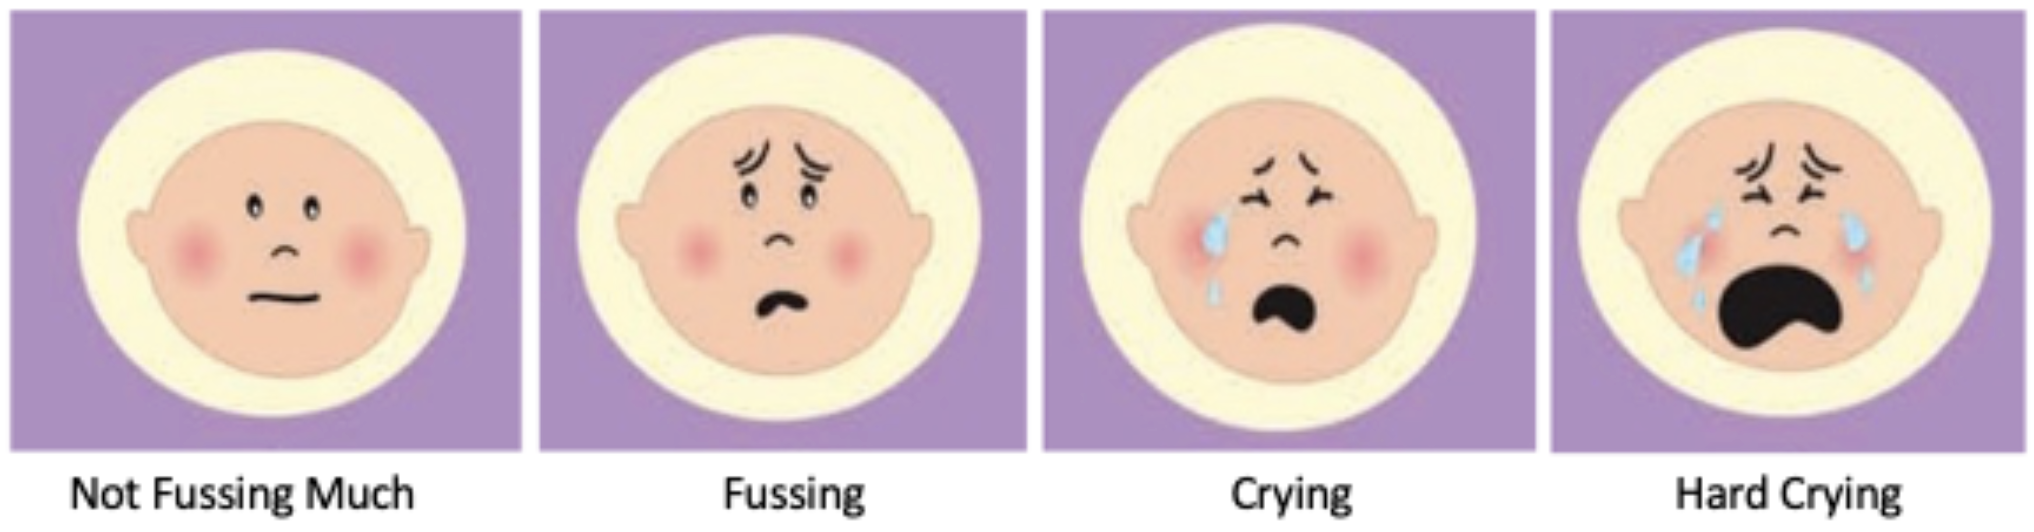
\includegraphics[width=0.5\textwidth,height=\textheight]{../viz/adams_scale.png}

\textbf{9.2.}{[}\emph{If baby was fussy}{]} \textbf{What did you do to
calm BABY down? {[}check all that apply{]}}

\begin{enumerate}
\def\labelenumi{\alph{enumi}.}
\tightlist
\item
  Feed
\item
  Rub or pat
\item
  Swaddle
\item
  Pick up/Bounce/rock/swing
\item
  Shush/white noise
\item
  Play TV/tablet/video/etc
\item
  Play recorded music
\item
  Sing
\item
  Give pacifier / teether
\item
  Put in bed
\item
  Change diaper
\item
  Waited for them to calm down
\item
  Other
\end{enumerate}

\textbf{9.3.} {[}\emph{If baby was fussy}{]} \textbf{How long did it
take BABY to calm down?}

\begin{enumerate}
\def\labelenumi{\alph{enumi}.}
\tightlist
\item
  Less than 1 minute
\item
  1-2 minutes
\item
  3-5 minutes
\item
  6-10 minutes
\item
  11-20 minutes
\item
  20+ minutes (or still fussing)
\end{enumerate}

\textbf{10. Did you sing to BABY in the last 2-3 hours?}

\begin{enumerate}
\def\labelenumi{\alph{enumi}.}
\tightlist
\item
  Yes
\item
  No
\end{enumerate}

\textbf{11. Have you played recorded music for BABY in the last 2-3
hours?}

\begin{enumerate}
\def\labelenumi{\alph{enumi}.}
\tightlist
\item
  Yes
\item
  No
\end{enumerate}

\textbf{12. Have you made or listened to music for your own enjoyment in
the last 2-3 hours?}

\begin{enumerate}
\def\labelenumi{\alph{enumi}.}
\tightlist
\item
  Yes
\item
  No
\end{enumerate}

\subsection*{Supplementary Text 3: Results from caregiver exit
survey}\label{supplementary-text-3-results-from-caregiver-exit-survey}
\addcontentsline{toc}{subsection}{Supplementary Text 3: Results from
caregiver exit survey}

At the end of the study, caregivers were invited to complete an optional
exit survey to share their overall experiences during the 10-week study
period. Fifty-eight caregivers (52.7\%) chose to do so. Summary
information from the survey is presented here.

\subsubsection*{Positive experiences in the
study}\label{positive-experiences-in-the-study}
\addcontentsline{toc}{subsubsection}{Positive experiences in the study}

The majority of respondents (89.7\%) described their experience
positively, typically mentioning opportunities to actively integrate
music into their daily lives, which they felt led to positive
experiences:

\begin{quote}
\textit{We had a lot of fun singing songs… there was one particular road trip that was challenging [and] I was inspired by the study to sing a lot on to help get us through.}
  
\textit{… She would smile when we sang if she would start to get fussy or be ready for bed. I think it cued her body that she was going to sleep or help soothe her. Really loved the experience! I also felt like the singing bonded us even more!}
  
\textit{I could definitely see that singing to my baby helped soothe him. I really enjoyed the experiment and will keep singing to my baby everyday.}
  
\textit{This study really brought more singing and song-play into my relationship with my son.}
  
\textit{[Baby] responded so well to the signing and would get really excited especially when you're really animated and do actions. It was also helpful when she was unsettled and would calm her quickly.}
  
\textit{[Baby] just loves songs and [it’s] part of our daily routine – I’m not sure if we would have sung as much if we didn’t do the study. She laughs and giggles and particularly loves songs with actions.}
  
\textit{For my own mental health, singing calmed me down and refreshed me almost whilst with my baby it definitely put a smile on her face.}
\end{quote}

\subsubsection*{Views on the music enrichment intervention
varied}\label{views-on-the-music-enrichment-intervention-varied}
\addcontentsline{toc}{subsubsection}{Views on the music enrichment
intervention varied}

Consistent with EMA results, most respondents (94.8\%) reported that
they were able to increase singing during the intervention period.
However, while many found the singing intervention materials helpful for
incorporating more singing into their daily routines, their reactions to
the types of material varied.

For example, less than half of the respondents (43.1\%) regularly used
the original songs we produced to broaden caregivers' repertoire for
singing to their infants. Some comments hinted at caregivers' preference
for singing familiar songs rather than learning new songs (e.g., ``I
would have preferred more common children's songs\ldots even if they
were in other languages''; ``I had plenty of my own songs''; ``Just not
my favorite, not very familiar'').

On the other hand, a large number of respondents liked (77.6\%) and
actively used the infant-friendly board book that was sent to
participants, which contained widely popular songs for infants (e.g.,
The Wheels on the Bus, Head Shoulders Knees \& Toes, Twinkle Twinkle
Little Star). The easy accessibility of this physical book (i.e., there
was no need to open and navigate their phone to access songs) also
seemed not only to add convenience for caregivers but also to attract
older siblings of their infants:

\begin{quote}
\textit{My 2yo loved getting involved with singing the songs in the board book!}
  
\textit{My older children enjoyed the board book and began to sing the songs to their sibling too.}
  
\textit{My older child loves the book and frequently uses it to sing with the baby.}
\end{quote}

\subsubsection*{Caregivers' ability to complete EMA surveys
varied}\label{caregivers-ability-to-complete-ema-surveys-varied}
\addcontentsline{toc}{subsubsection}{Caregivers' ability to complete EMA
surveys varied}

Some participants found it challenging to respond promptly upon
receiving an EMA ping (34.5\%). When asked to suggest the ideal time for
EMA surveys, 19 respondents recommended when their infants are asleep
(e.g., naptime, nighttime), although, of course, this would be
scientifically counterproductive, in that responses would be
retrospective.

Some parents also noted that due to the complexity of daily life with
young infants, caregivers sometimes had to delay completing surveys
until they had spare moments to complete, even if they noticed the EMA
ping at the moment. There were also instances when caregivers found the
EMA ping had expired at the time when they found a moment to fill out
the survey:

\begin{quote}
\textit{Generally, I responded within 2-4 hrs, as I couldn't guarantee 2 minutes un-interrupted until then.}
  
\textit{Unfortunately the time lapsed on some and was just too busy and would forget to go back to it.}
  
\textit{Difficult juggling baby so sometimes forgot to return once started.}
  
\textit{I didn’t notice the notifications until it was too late and the survey had expired. I wish there was a bigger time window or to notify more prominently.}
  
\textit{It would be good to have more than 4 hours before the survey expired as I wasn't always to complete the survey in that timeframe.}
  
\end{quote}

These responses highlight the challenges caregivers face in promptly
responding to EMA pings while caring for their infants, suggesting the
need for careful consideration in determining EMA schedules.
Nonetheless, the high compliance rate found in the current study,
despite the study asking caregivers to respond to nearly 100 surveys in
10 weeks, suggests that EMA may be a promising method to adopt in
studies of other naturalistic behaviors, especially those amenable to
longitudinal study.

\clearpage

\subsection*{Supplementary Figures}\label{supplementary-figures}
\addcontentsline{toc}{subsection}{Supplementary Figures}

\begin{figure}[H]

{\centering 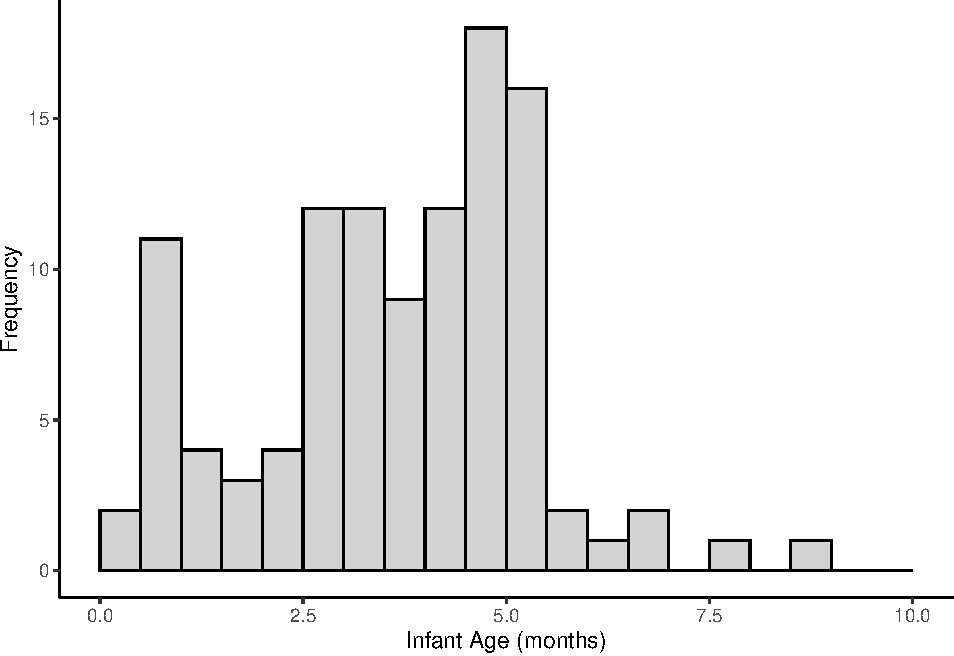
\includegraphics[width=1\linewidth,]{MIPH_childdev_files/figure-latex/supp figure 1-1} 

}

\caption{\textbf{Supplementary Figure 1 | Histogram of infant ages at the start of the study.}}\label{fig:supp figure 1}
\end{figure}
\clearpage

\begin{figure}[H]

{\centering 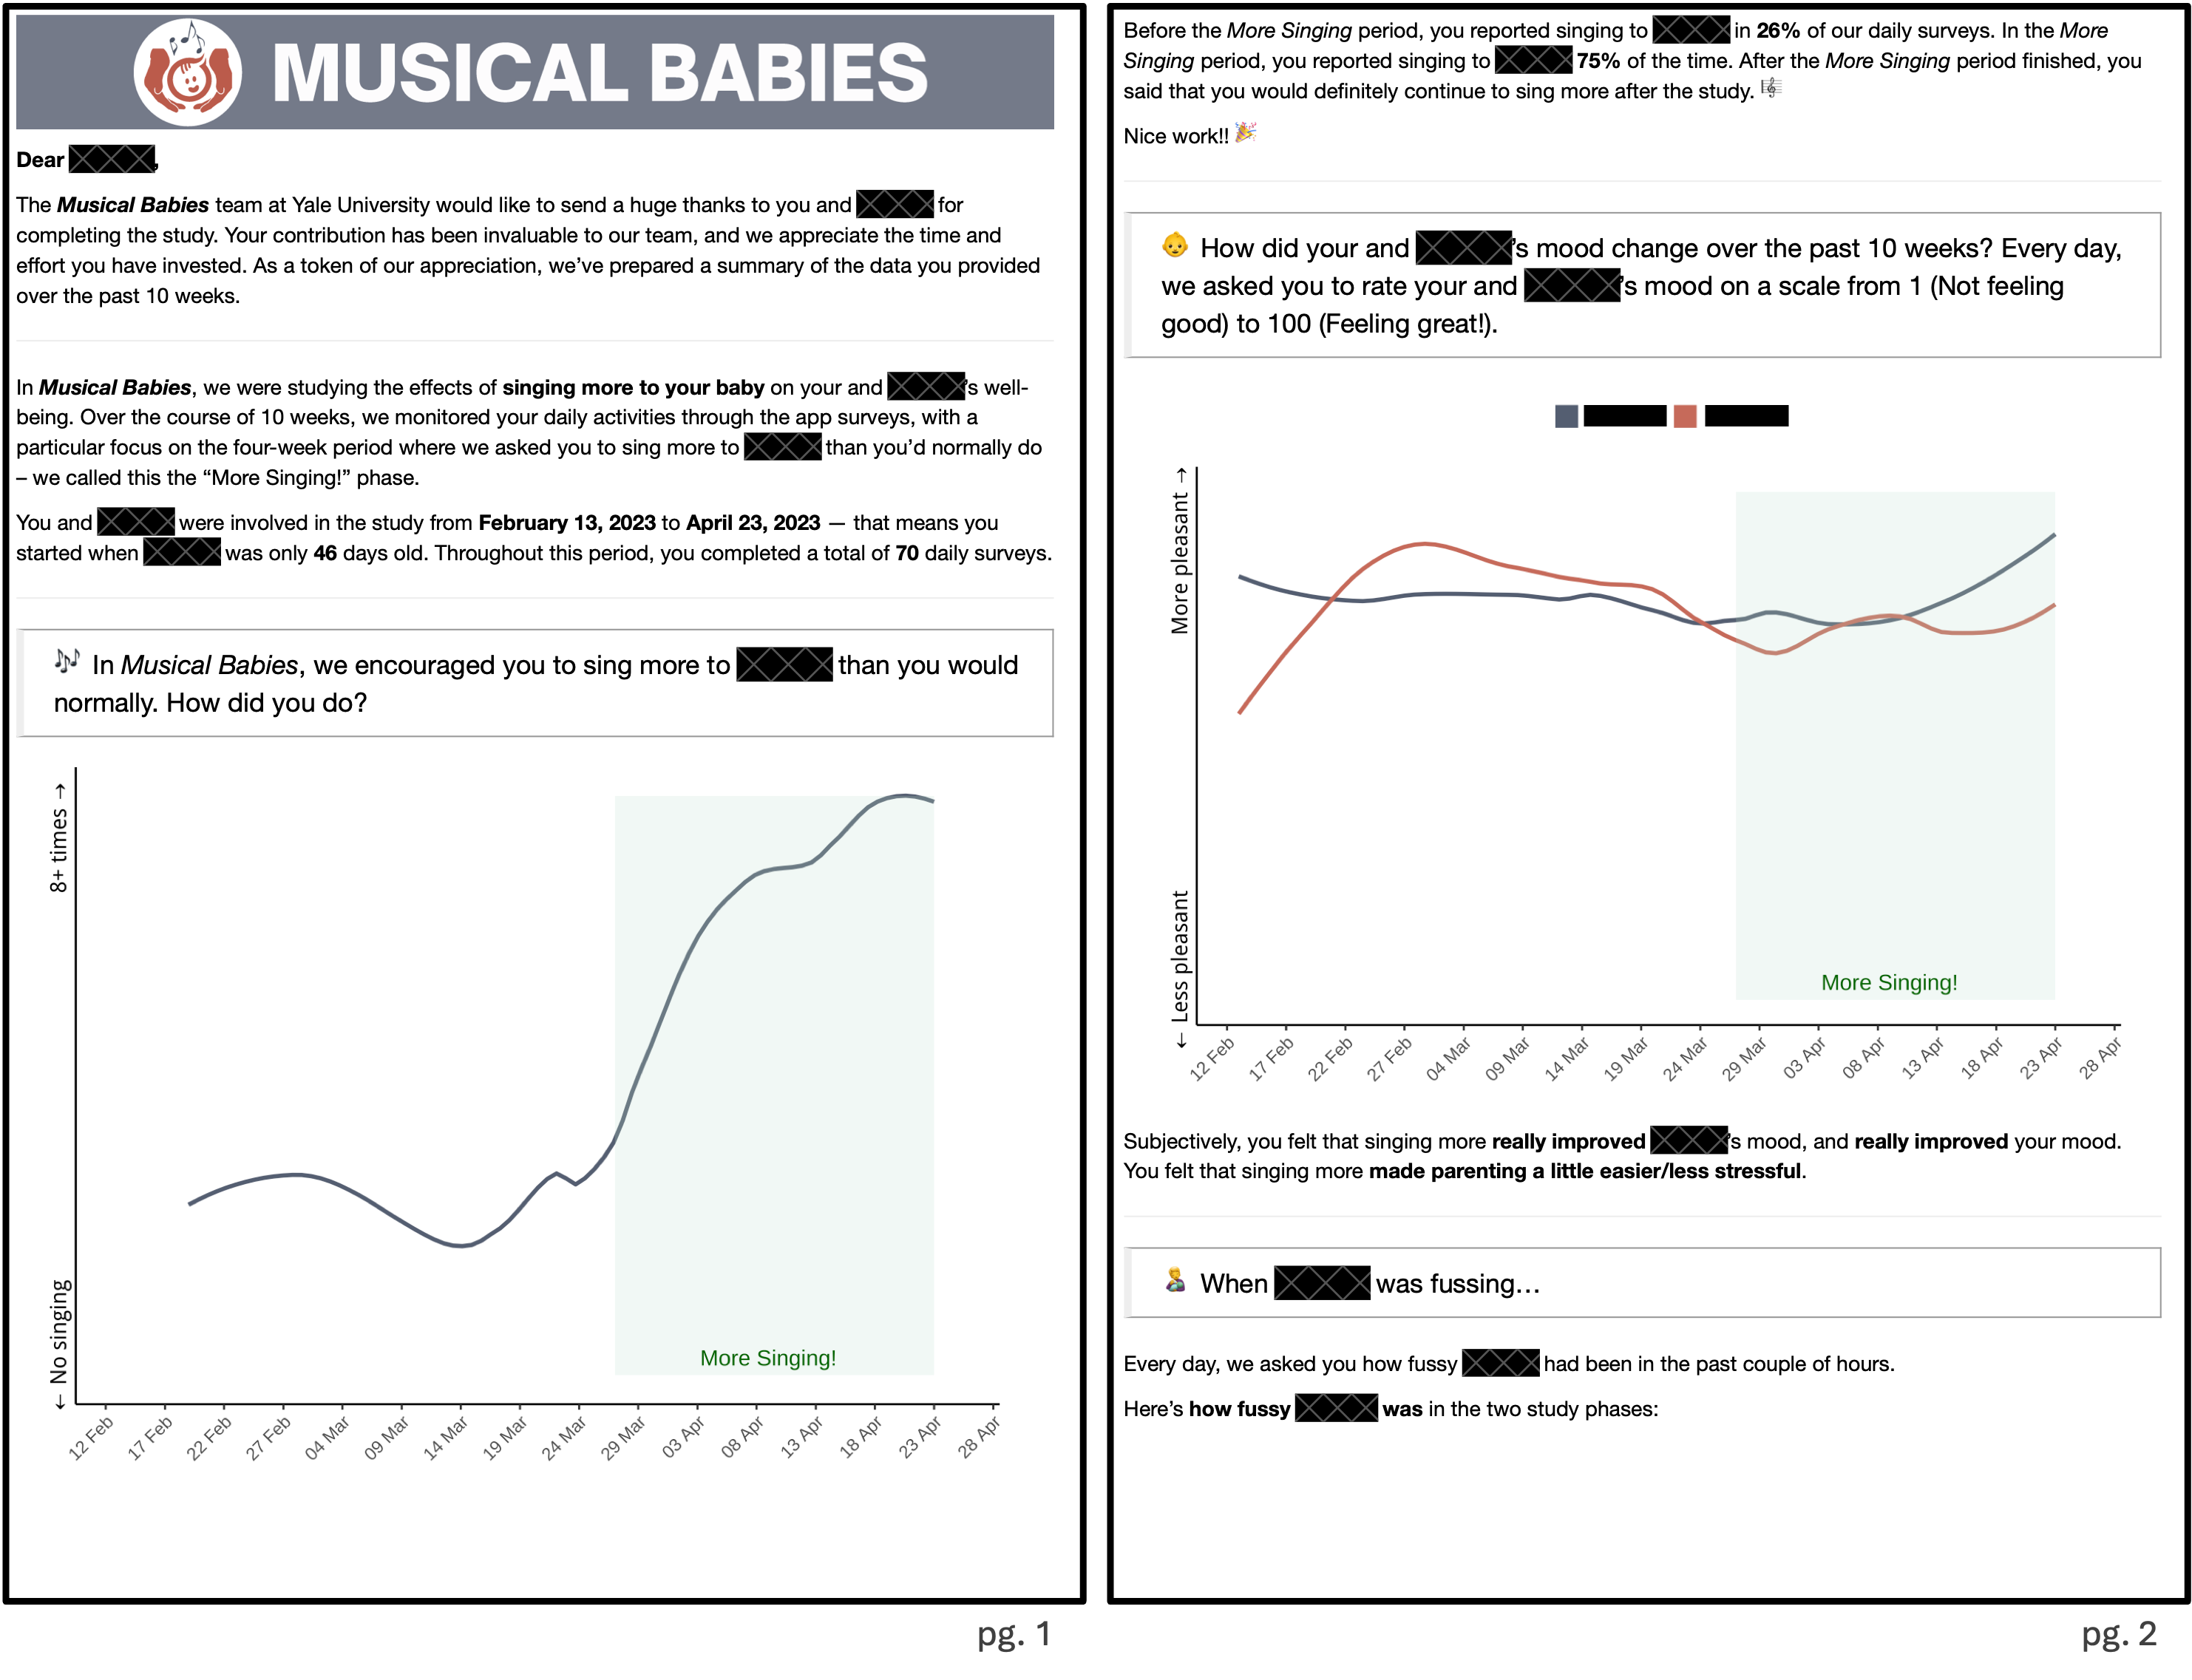
\includegraphics[width=0.9\linewidth,]{../viz/s_figure2a} 

}

\caption{\textbf{Supplementary Figure 2 | Example report for participants.} At the end of the study, we sent participants a report summarizing data they provided over the course of the study, as an incentive.}\label{fig:supp fig 2}
\end{figure}
\begin{figure}[H]

{\centering 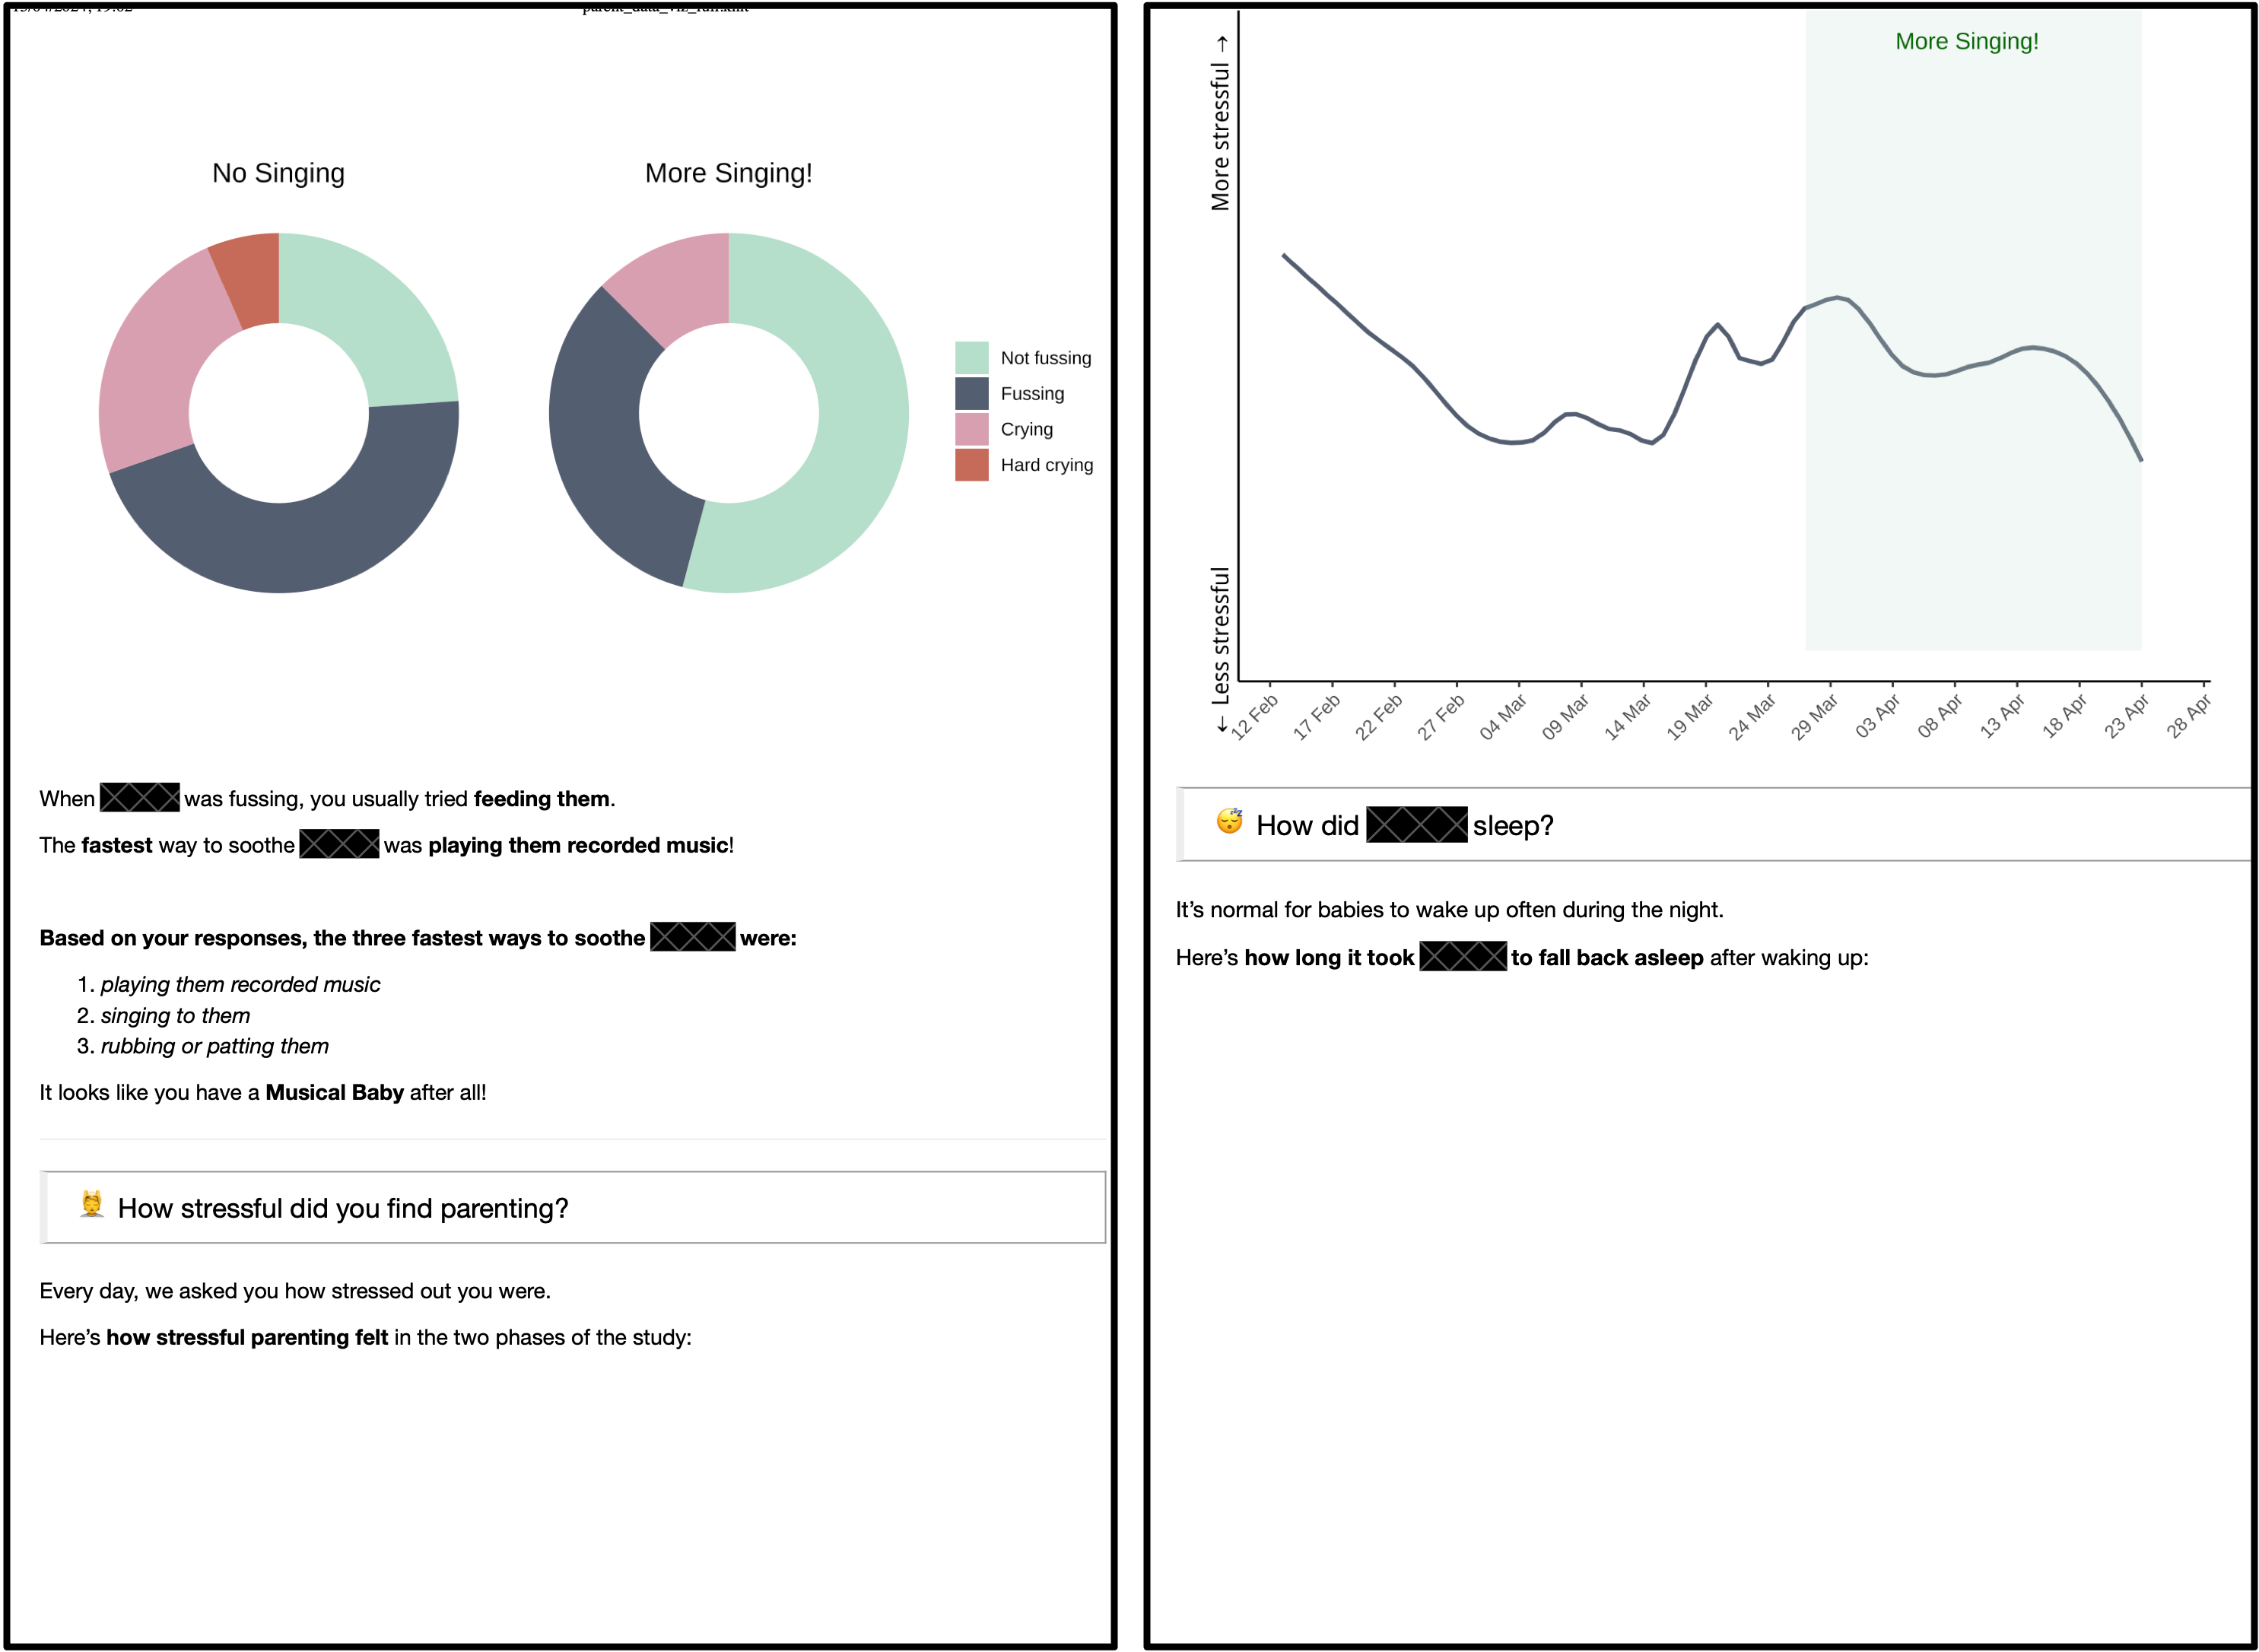
\includegraphics[width=0.9\linewidth,]{../viz/s_figure2b} 

}

\caption{\textbf{Supplementary Figure 2 (cont.) | Example report for participants.}}\label{fig:supp fig 2b}
\end{figure}

\begin{figure}[H]

{\centering 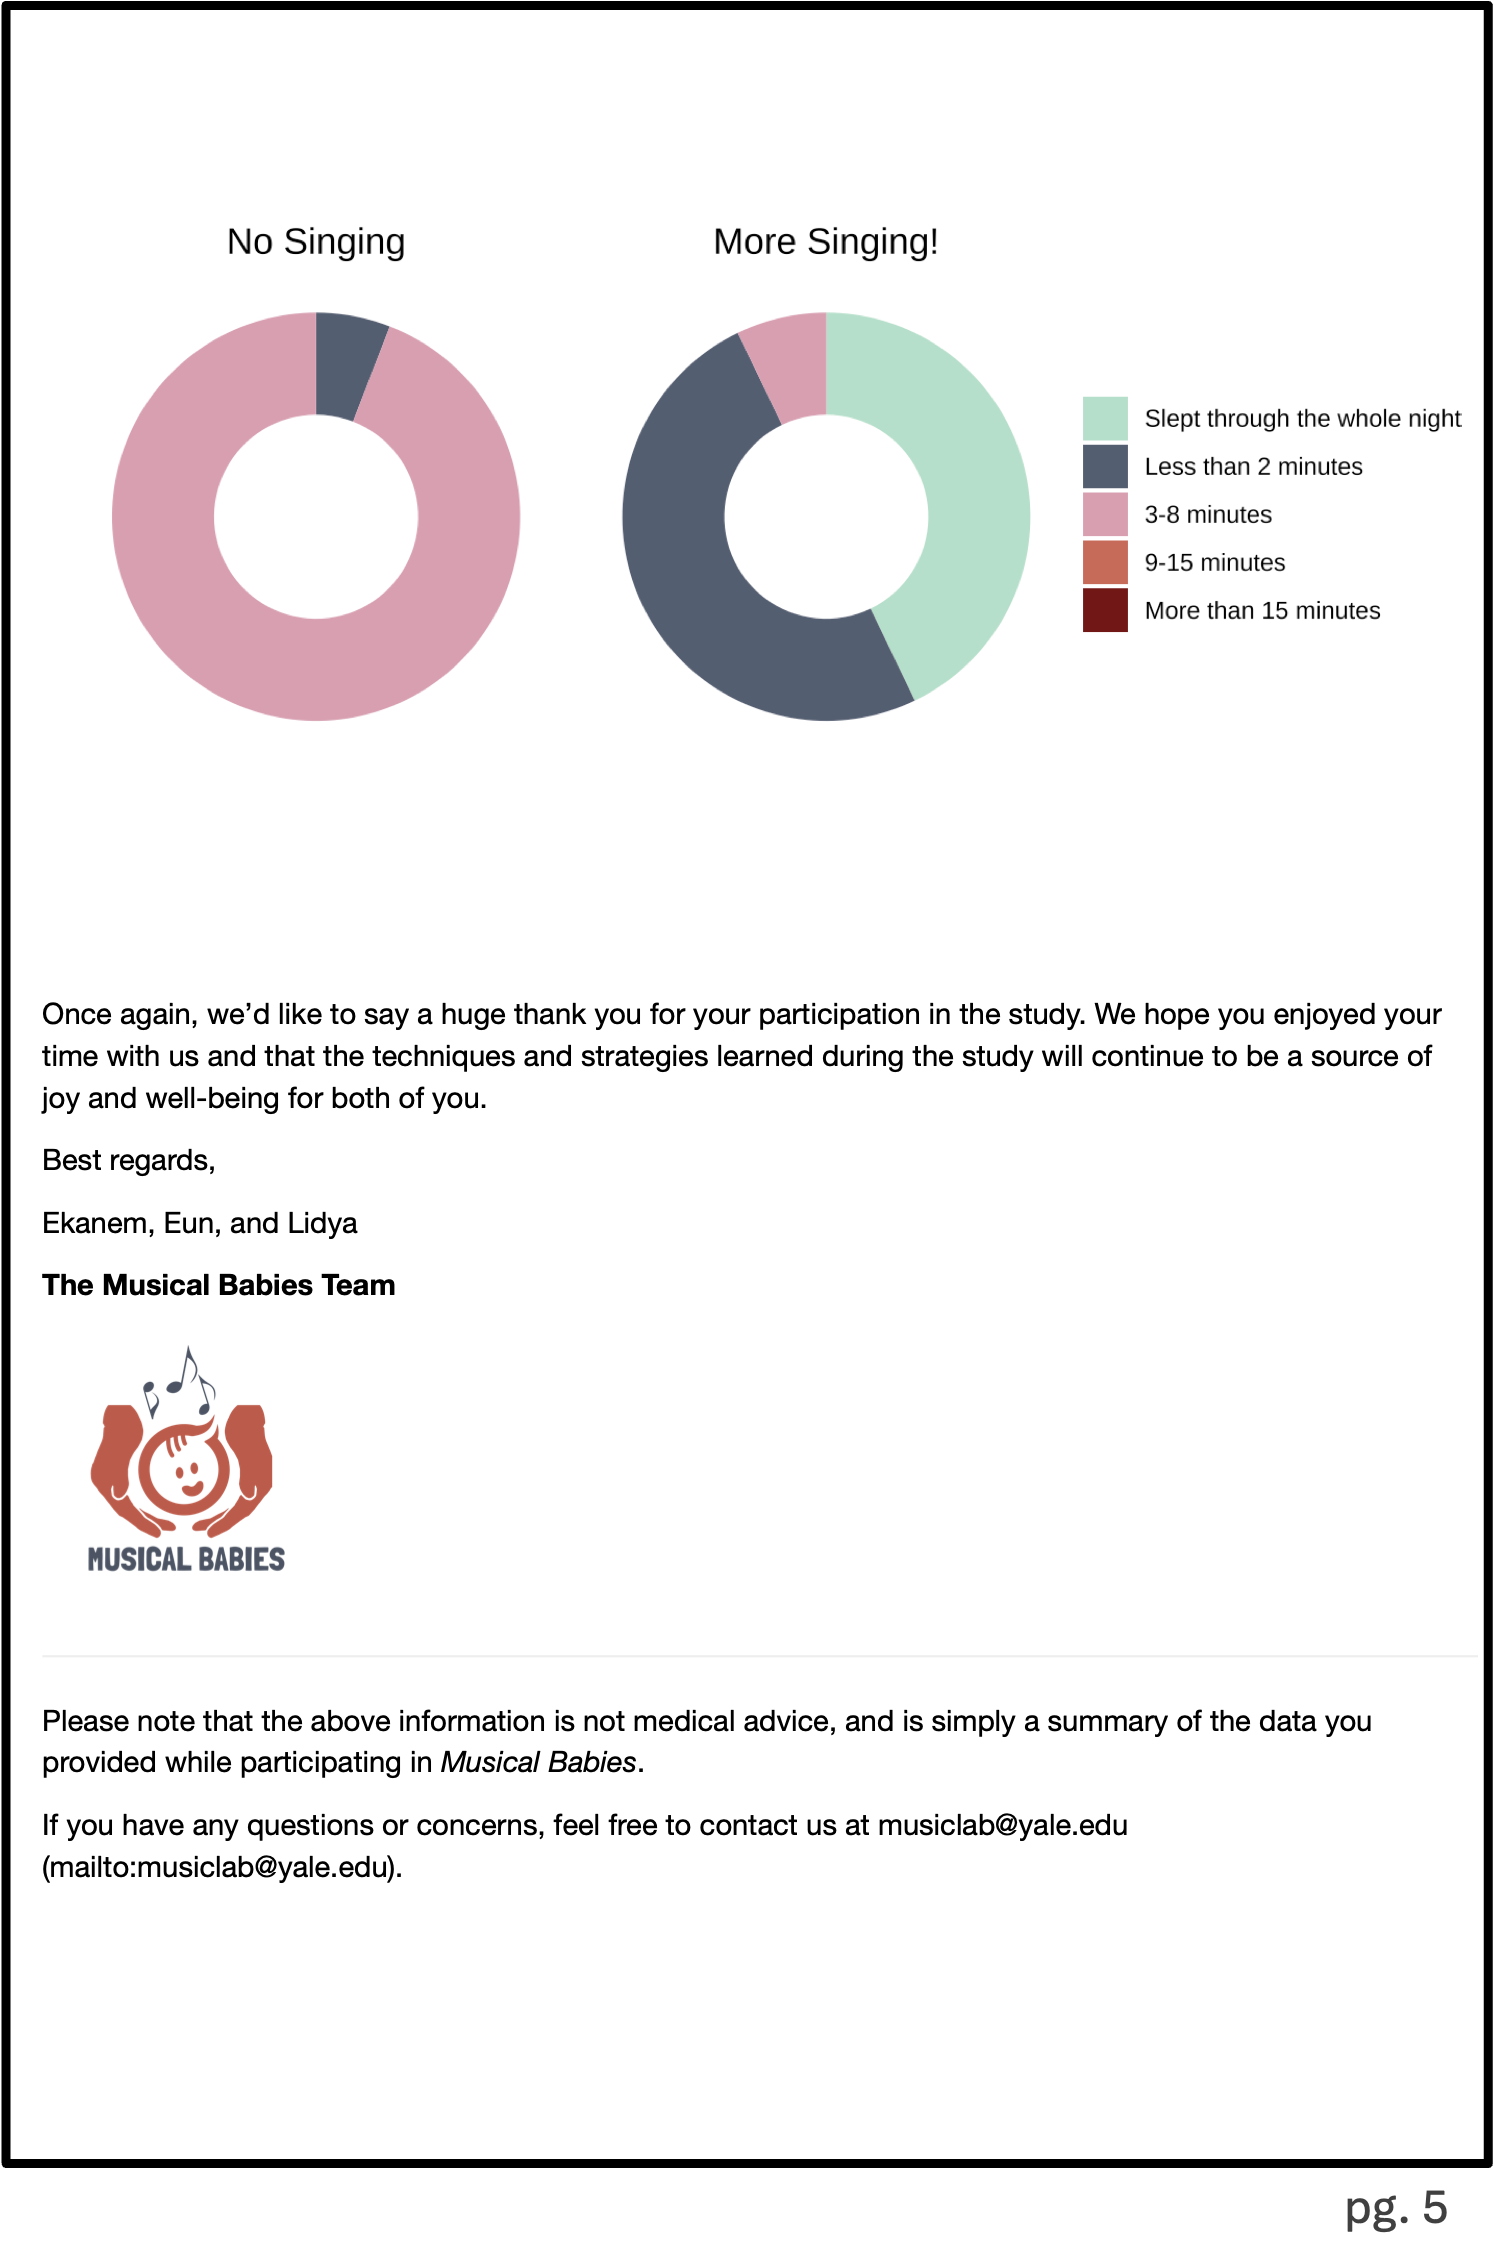
\includegraphics[width=0.5\linewidth,]{../viz/s_figure2c} 

}

\caption{\textbf{Supplementary Figure 2 (cont.) | Example report for participants.}}\label{fig:supp fig 2c}
\end{figure}

\clearpage

\subsection*{Supplementary Tables}\label{supplementary-tables}
\addcontentsline{toc}{subsection}{Supplementary Tables}

\begin{ThreePartTable}
\begin{TableNotes}[para]
\item \textbf{Supplementary Table 1 | Participants' musical backgrounds.} 
\item We measured participants' level of musical training with the question "How would you describe your music training experience?". Participants could select any of the following types of musical training: no formal musical training, lessons or classes (either before or during elementary school years, during middle and high school years, or in adulthood), participation in community-based music groups (e.g.,  church choir, community ensembles), majoring in music, and a free-text option. Partipants who reported either majoring or minoring in music, or working in music professionally were coded as having an "advanced" background in music. We then counted the number of other responses (excluding "no formal musical training") selected by each participant, and coded participants as having either "some" (< 2 categories selected) or "intermediate" (< 4 categories selected) training in music.
\end{TableNotes}
\begin{longtable}{lrl}
\toprule
Level of music training & n & \% of sample\\
\midrule
Advanced & 14 & 13.00\\
\cmidrule{1-3}\pagebreak[0]
Intermediate & 15 & 14.00\\
\cmidrule{1-3}\pagebreak[0]
Some & 62 & 56.00\\
\cmidrule{1-3}\pagebreak[0]
None & 18 & 16.00\\
\bottomrule
\insertTableNotes
\end{longtable}
\end{ThreePartTable}
\clearpage

\section*{References}\label{references}
\addcontentsline{toc}{section}{References}

\phantomsection\label{refs}
\begin{CSLReferences}{1}{0}
\bibitem[\citeproctext]{ref-Adams2019}
Adams, E. L., Marini, M. E., Brick, T. R., Paul, I. M., Birch, L. L., \&
Savage, J. S. (2019). Ecological momentary assessment of using food to
soothe during infancy in the {INSIGHT} trial. \emph{International
Journal of Behavioral Nutrition and Physical Activity}, \emph{16}(1),
79. \url{https://doi.org/10.1186/s12966-019-0837-y}

\bibitem[\citeproctext]{ref-Allen2018}
Allen, A., Tosun, N., Carlson, S., \& Allen, S. (2018). Postpartum
{Changes} in {Mood} and {Smoking}-{Related} {Symptomatology}: {An}
{Ecological} {Momentary} {Assessment} {Investigation}. \emph{Nicotine \&
Tobacco Research}, \emph{20}(6), 681--689.
\url{https://doi.org/10.1093/ntr/ntx118}

\bibitem[\citeproctext]{ref-Arnon2014}
Arnon, S., Diamant, C., Bauer, S., Regev, R., Sirota, G., \&
Litmanovitz, I. (2014). Maternal singing during kangaroo care led to
autonomic stability in preterm infants and reduced maternal anxiety.
\emph{Acta Paediatrica}, \emph{103}(10), 1039--1044.
\url{https://doi.org/10.1111/apa.12744}

\bibitem[\citeproctext]{ref-Bainbridge2021}
Bainbridge, C. M., Bertolo, M., Youngers, J., Atwood, S., Yurdum, L.,
Simson, J., Lopez, K., Xing, F., Martin, A., \& Mehr, S. A. (2021).
Infants relax in response to unfamiliar foreign lullabies. \emph{Nature
Human Behaviour}. \url{https://doi.org/10.1038/s41562-020-00963-z}

\bibitem[\citeproctext]{ref-deBarbaro2023}
Barbaro, K. de, Micheletti, M., Yao, X., Khante, P., Johnson, M., \&
Goodman, S. (2023). Infant crying predicts real-time fluctuations in
maternal mental health in ecologically valid home settings.
\emph{Developmental Psychology}, \emph{59}(4), 733--744.
\url{https://doi.org/10.1037/dev0001530}

\bibitem[\citeproctext]{ref-Barr1990}
Barr, R. G. (1990). The {Normal Crying Curve}: {What Do We Really Know}?
\emph{Developmental Medicine \& Child Neurology}, \emph{32}(4),
356--362. \url{https://doi.org/10.1111/j.1469-8749.1990.tb16949.x}

\bibitem[\citeproctext]{ref-Bowlby1969}
Bowlby, J. (1969). \emph{Attachment and loss ({Vol}. {I}:
{Attachment})}. Basic Books.

\bibitem[\citeproctext]{ref-Cheng2023}
Cheng, Q., Roth, A., Halgren, E., Klein, D., Chen, J.-K., \& Mayberry,
R. I. (2023). Restricted language access during childhood affects adult
brain structure in selective language regions. \emph{Proceedings of the
National Academy of Sciences}, \emph{120}(7), e2215423120.
\url{https://doi.org/10.1073/pnas.2215423120}

\bibitem[\citeproctext]{ref-Cho2021}
Cho, E., \& Ilari, B. S. (2021). Mothers as home {DJs}: {Recorded} music
and young children's well-being during the {Covid}-19 pandemic.
\emph{Frontiers in Psychology}, \emph{12}, 637569.
\url{https://doi.org/10.3389/fpsyg.2021.637569}

\bibitem[\citeproctext]{ref-Cirelli2019}
Cirelli, L. K., Jurewicz, Z. B., \& Trehub, S. E. (2019). Effects of
maternal singing style on mother--infant arousal and behavior.
\emph{Journal of Cognitive Neuroscience}.
\url{https://doi.org/10.1162/jocn_a_01402}

\bibitem[\citeproctext]{ref-Cirelli2020b}
Cirelli, L. K., Jurewicz, Z. B., \& Trehub, S. E. (2020). Effects of
maternal singing style on mother-infant arousal and behavior.
\emph{Journal of Cognitive Neuroscience}, \emph{32}(7), 1213--1220.
\url{https://doi.org/10.1162/jocn_a_01402}

\bibitem[\citeproctext]{ref-Cirelli2020}
Cirelli, L. K., \& Trehub, S. E. (2020). Familiar songs reduce infant
distress. \emph{Developmental Psychology}.
\url{https://doi.org/10.1037/dev0000917}

\bibitem[\citeproctext]{ref-Corbeil2016}
Corbeil, M., Trehub, S. E., \& Peretz, I. (2016). Singing delays the
onset of infant distress. \emph{Infancy}, \emph{21}(3), 373--391.
\url{https://doi.org/10.1111/infa.12114}

\bibitem[\citeproctext]{ref-Corpuz2023}
Corpuz, R., Kotov, D. A., \& Donovan, R. L. (2023). Earlier sexual debut
predicts higher (not lower) levels of father care measured across 12
weeks: An experience sampling study. \emph{Frontiers in Psychology},
\emph{14}, 1199735. \url{https://doi.org/10.3389/fpsyg.2023.1199735}

\bibitem[\citeproctext]{ref-Costa-Giomi2014}
Costa-Giomi, E., \& Ilari, B. (2014). Infants' preferential attention to
sung and spoken stimuli. \emph{Journal of Research in Music Education},
\emph{62}(2), 188--194. \url{https://doi.org/10.1177/0022429414530564}

\bibitem[\citeproctext]{ref-Custodero2003}
Custodero, L. A., Rebello Britto, P., \& Brooks-Gunn, J. (2003). Musical
lives: {A} collective portrait of {American} parents and their young
children. \emph{Journal of Applied Developmental Psychology},
\emph{24}(5), 553--572.
\url{https://doi.org/10.1016/j.appdev.2003.08.005}

\bibitem[\citeproctext]{ref-Davis2004}
Davis, E. P., Snidman, N., Wadhwa, P. D., Glynn, L. M., Schetter, C. D.,
\& Sandman, C. A. (2004). Prenatal maternal anxiety and depression
predict negative behavioral reactivity in infancy. \emph{Infancy},
\emph{6}(3), 319--331. \url{https://doi.org/10.1207/s15327078in0603_1}

\bibitem[\citeproctext]{ref-Dennis2006}
Dennis, C.-L., \& Ross, L. (2006). Women's perceptions of partner
support and conflict in the development of postpartum depressive
symptoms. \emph{Journal of Advanced Nursing}, \emph{56}(6), 588--599.
\url{https://doi.org/10.1111/j.1365-2648.2006.04059.x}

\bibitem[\citeproctext]{ref-Dora2024}
Dora, J., Kuczynski, A. M., Schultz, M. E., Acuff, S. F., Murphy, J. G.,
\& King, K. M. (2024). An experimental investigation into the effect of
negative affect on the behavioral economic demand for alcohol.
\emph{Psychology of Addictive Behaviors}.
\url{https://psycnet.apa.org/record/2024-42616-001}

\bibitem[\citeproctext]{ref-Fancourt2017}
Fancourt, D., \& Perkins, R. (2017). Maternal engagement with music up
to nine months post-birth: {Findings} from a cross-sectional study in
{England}. \emph{Psychology of Music}, 0305735617705720.
\url{https://doi.org/10.1177/0305735617705720}

\bibitem[\citeproctext]{ref-Fancourt2018}
Fancourt, D., \& Perkins, R. (2018a). Effect of singing interventions on
symptoms of postnatal depression: Three-arm randomised controlled trial.
\emph{The British Journal of Psychiatry}, 1--3.
\url{https://doi.org/10.1192/bjp.2017.29}

\bibitem[\citeproctext]{ref-Fancourt2018a}
Fancourt, D., \& Perkins, R. (2018b). Could listening to music during
pregnancy be protective against postnatal depression and poor wellbeing
post birth? {Longitudinal} associations from a preliminary prospective
cohort study. \emph{BMJ Open}, \emph{8}(7), e021251.
\url{https://doi.org/10.1136/bmjopen-2017-021251}

\bibitem[\citeproctext]{ref-Feldman2009}
Feldman, R., Granat, A., Pariente, C., Kanety, H., Kuint, J., \&
Gilboa-Schechtman, E. (2009). Maternal depression and anxiety across the
postpartum year and infant social engagement, fear regulation, and
stress reactivity. \emph{Journal of the American Academy of Child \&
Adolescent Psychiatry}, \emph{48}(9), 919--927.
\url{https://doi.org/10.1097/CHI.0b013e3181b21651}

\bibitem[\citeproctext]{ref-Feldman1999}
Feldman, R., Greenbaum, C. W., \& Yirmiya, N. (1999). Mother--infant
affect synchrony as an antecedent of the emergence of self-control.
\emph{Developmental Psychology}, \emph{35}(1), 223--231.
\url{https://doi.org/10.1037/0012-1649.35.1.223}

\bibitem[\citeproctext]{ref-Feldman2014}
Feldman, R., Rosenthal, Z., \& Eidelman, A. I. (2014). Maternal-preterm
skin-to-skin contact enhances child physiologic organization and
cognitive control across the first 10 years of life. \emph{Biological
Psychiatry}, \emph{75}(1), 56--64.
\url{https://doi.org/10.1016/j.biopsych.2013.08.012}

\bibitem[\citeproctext]{ref-Fernald2013}
Fernald, A., Marchman, V. A., \& Weisleder, A. (2013). {SES} differences
in language processing skill and vocabulary are evident at 18 months.
\emph{Developmental Science}, \emph{16}(2), 234--248.
\url{https://doi.org/10.1111/desc.12019}

\bibitem[\citeproctext]{ref-Filippa2013}
Filippa, M., Devouche, E., Arioni, C., Imberty, M., \& Gratier, M.
(2013). Live maternal speech and singing have beneficial effects on
hospitalized preterm infants. \emph{Acta Paediatrica}, \emph{102}(10),
1017--1020. \url{https://doi.org/10.1111/apa.12356}

\bibitem[\citeproctext]{ref-Franchak2019}
Franchak, J. M. (2019). Changing {Opportunities} for {Learning} in
{Everyday} {Life}: {Infant} {Body} {Position} {Over} the {First} {Year}.
\emph{Infancy}, \emph{24}(2), 187--209.
\url{https://doi.org/10.1111/infa.12272}

\bibitem[\citeproctext]{ref-Franchak2024}
Franchak, J. M., Kadooka, K., \& Fausey, C. M. (2024). Longitudinal
relations between independent walking, body position, and object
experiences in home life. \emph{Developmental Psychology}, \emph{60}(2),
228--242. \url{https://doi.org/10.1037/dev0001678}

\bibitem[\citeproctext]{ref-Fries2005}
Fries, A. B. W., Ziegler, T. E., Kurian, J. R., Jacoris, S., \& Pollak,
S. D. (2005). Early experience in humans is associated with changes in
neuropeptides critical for regulating social behavior. \emph{Proceedings
of the National Academy of Sciences}, \emph{102}(47), 17237--17240.
\url{https://doi.org/10.1073/pnas.0504767102}

\bibitem[\citeproctext]{ref-Hemmerechts2017}
Hemmerechts, K., Agirdag, O., \& Kavadias, D. (2017). The relationship
between parental literacy involvement, socio-economic status and reading
literacy. \emph{Educational Review}, \emph{69}(1), 85--101.
\url{https://doi.org/10.1080/00131911.2016.1164667}

\bibitem[\citeproctext]{ref-Hilton2022a}
Hilton, C. B., Moser, C. J., Bertolo, M., Lee-Rubin, H., Amir, D.,
Bainbridge, C. M., Simson, J., Knox, D., Glowacki, L., Alemu, E.,
Galbarczyk, A., Jasienska, G., Ross, C. T., Neff, M. B., Martin, A.,
Cirelli, L. K., Trehub, S. E., Song, J., Kim, M., \ldots{} Mehr, S. A.
(2022). Acoustic regularities in infant-directed speech and song across
cultures. \emph{Nature Human Behaviour}.
\url{https://doi.org/10.1101/2020.04.09.032995}

\bibitem[\citeproctext]{ref-Kotler2019}
Kotler, J., Mehr, S. A., Egner, A., Haig, D., \& Krasnow, M. M. (2019).
Response to vocal music in {Angelman} syndrome contrasts with
{Prader}-{Willi} syndrome. \emph{Evolution and Human Behavior},
\emph{40}(5), 420--426.
\url{https://doi.org/10.1016/j.evolhumbehav.2019.05.003}

\bibitem[\citeproctext]{ref-Kuczynski2023}
Kuczynski, A. M., Piccirillo, M., Dora, J., Kuehn, K. S., Halvorson, M.
A., King, K. M., \& Kanter, J. (2023). \emph{Characterizing the
{Momentary} {Association} {Between} {Loneliness}, {Depression}, and
{Social} {Interactions}: {Insights} from an {Ecological} {Momentary}
{Assessment} {Study}}. \url{https://osf.io/btwk8/download}

\bibitem[\citeproctext]{ref-Lense2022}
Lense, M. D., Shultz, S., Astésano, C., \& Jones, W. (2022). Music of
infant-directed singing entrains infants' social visual behavior.
\emph{Proceedings of the National Academy of Sciences}, \emph{119}(45),
e2116967119. \url{https://doi.org/10.1073/pnas.2116967119}

\bibitem[\citeproctext]{ref-Liu2023}
Liu, J., Hilton, C. B., Bergelson, E., \& Mehr, S. A. (2023). Language
experience predicts music processing in a half-million speakers of
fifty-four languages. \emph{Current Biology}, \emph{33}(10),
1916--1925.e4. \url{https://doi.org/10.1016/j.cub.2023.03.067}

\bibitem[\citeproctext]{ref-Long2023}
Long, B., Simson, J., Buxó-Lugo, A., Watson, D. G., \& Mehr, S. A.
(2023). How games can make behavioural science better. \emph{Nature},
\emph{613}(7944), 433--436.
\url{https://doi.org/10.1038/d41586-023-00065-6}

\bibitem[\citeproctext]{ref-Malloch1999}
Malloch, S. N. (1999). Mothers and infants and communicative musicality.
\emph{Musicae Scientiae}, \emph{3}(1\_suppl), 29--57.
\url{https://doi.org/10.1177/10298649000030S104}

\bibitem[\citeproctext]{ref-Malloch2009}
Malloch, S. N., \& Trevarthen, C. (2009). \emph{Communicative
musicality: Exploring the basis of human companionship}. Oxford
University Press.

\bibitem[\citeproctext]{ref-Mehr2014}
Mehr, S. A. (2014). Music in the home: {New} evidence for an
intergenerational link. \emph{Journal of Research in Music Education},
\emph{62}(1), 78--88. \url{https://doi.org/10.1177/0022429413520008}

\bibitem[\citeproctext]{ref-Mehr2017a}
Mehr, S. A., Kotler, J., Howard, R. M., Haig, D., \& Krasnow, M. M.
(2017). Genomic imprinting is implicated in the psychology of music.
\emph{Psychological Science}, \emph{28}(10), 1455--1467.
\url{https://doi.org/10.1177/0956797617711456}

\bibitem[\citeproctext]{ref-Mehr2017}
Mehr, S. A., \& Krasnow, M. M. (2017). Parent-offspring conflict and the
evolution of infant-directed song. \emph{Evolution and Human Behavior},
\emph{38}(5), 674--684.
\url{https://doi.org/10.1016/j.evolhumbehav.2016.12.005}

\bibitem[\citeproctext]{ref-Mehr2021}
Mehr, S. A., Krasnow, M. M., Bryant, G. A., \& Hagen, E. H. (2021).
Origins of music in credible signaling. \emph{Behavioral and Brain
Sciences}, \emph{44}, e60.
\url{https://doi.org/10.1017/S0140525X20000345}

\bibitem[\citeproctext]{ref-Mehr2019a}
Mehr, S. A., Singh, M., Knox, D., Ketter, D. M., Pickens-Jones, D.,
Atwood, S., Lucas, C., Jacoby, N., Egner, A. A., Hopkins, E. J., Howard,
R. M., Hartshorne, J. K., Jennings, M. V., Simson, J., Bainbridge, C.
M., Pinker, S., O'Donnell, T. J., Krasnow, M. M., \& Glowacki, L.
(2019). Universality and diversity in human song. \emph{Science},
\emph{366}(6468), 957--970. \url{https://doi.org/10.31234/osf.io/emq8r}

\bibitem[\citeproctext]{ref-Mehr2016}
Mehr, S. A., Song, L. A., \& Spelke, E. S. (2016). For 5-month-old
infants, melodies are social. \emph{Psychological Science},
\emph{27}(4), 486--501. \url{https://doi.org/10.1177/0956797615626691}

\bibitem[\citeproctext]{ref-Mehr2017b}
Mehr, S. A., \& Spelke, E. S. (2017). Shared musical knowledge in
11‐month‐old infants. \emph{Developmental Science}, \emph{21}(2).
\url{https://doi.org/10.1111/desc.12542}

\bibitem[\citeproctext]{ref-Moore2012}
Moore, E. R., Anderson, G. C., Bergman, N., \& Dowswell, T. (2012).
Early skin-to-skin contact for mothers and their healthy newborn
infants. In The Cochrane Collaboration (Ed.), \emph{Cochrane {Database}
of {Systematic} {Reviews}} (p. CD003519.pub3). John Wiley \& Sons, Ltd.
\url{https://doi.org/10.1002/14651858.CD003519.pub3}

\bibitem[\citeproctext]{ref-Nakata2004}
Nakata, T., \& Trehub, S. E. (2004). Infants' responsiveness to maternal
speech and singing. \emph{Infant Behavior and Development},
\emph{27}(4), 455--464.
\url{https://doi.org/10.1016/j.infbeh.2004.03.002}

\bibitem[\citeproctext]{ref-Nelson2007}
Nelson, C. A., Zeanah, C. H., Fox, N. A., Marshall, P. J., Smyke, A. T.,
\& Guthrie, D. (2007). Cognitive recovery in socially deprived young
children: {The} {Bucharest} early intervention project. \emph{Science},
\emph{318}(5858), 1937--1940.
\url{https://doi.org/10.1126/science.1143921}

\bibitem[\citeproctext]{ref-NICHDEarlyChildCareResearchNetwork2006}
NICHD Early Child Care Research Network. (2006). Infant-mother
attachment classification: {Risk} and protection in relation to changing
maternal caregiving quality. \emph{Developmental Psychology},
\emph{42}(1), 38--58. \url{https://doi.org/10.1037/0012-1649.42.1.38}

\bibitem[\citeproctext]{ref-Nolvi2016}
Nolvi, S., Karlsson, L., Bridgett, D. J., Pajulo, M., Tolvanen, M., \&
Karlsson, H. (2016). Maternal postnatal psychiatric symptoms and infant
temperament affect early mother-infant bonding. \emph{Infant Behavior
and Development}, \emph{43}, 13--23.
\url{https://doi.org/10.1016/j.infbeh.2016.03.003}

\bibitem[\citeproctext]{ref-Oddi2013}
Oddi, K. B., Murdock, K. W., Vadnais, S., Bridgett, D. J., \& Gartstein,
M. A. (2013). Maternal and {Infant} {Temperament} {Characteristics} as
{Contributors} to {Parenting} {Stress} in the {First} {Year}
{Postpartum}. \emph{Infant and Child Development}, \emph{22}(6),
553--579. \url{https://doi.org/10.1002/icd.1813}

\bibitem[\citeproctext]{ref-PascoFearon2011}
Pasco Fearon, R. M., \& Belsky, J. (2011). Infant-mother attachment and
the growth of externalizing problems across the primary-school years:
{Attachment} and externalizing problems. \emph{Journal of Child
Psychology and Psychiatry}, \emph{52}(7), 782--791.
\url{https://doi.org/10.1111/j.1469-7610.2010.02350.x}

\bibitem[\citeproctext]{ref-Puig2013}
Puig, J., Englund, M. M., Simpson, J. A., \& Collins, W. A. (2013).
Predicting adult physical illness from infant attachment: {A}
prospective longitudinal study. \emph{Health Psychology}, \emph{32}(4),
409--417. \url{https://doi.org/10.1037/a0028889}

\bibitem[\citeproctext]{ref-Reid2015}
Reid, K. M., \& Taylor, M. G. (2015). Social support, stress, and
maternal postpartum depression: {A} comparison of supportive
relationships. \emph{Social Science Research}, \emph{54}, 246--262.
\url{https://doi.org/10.1016/j.ssresearch.2015.08.009}

\bibitem[\citeproctext]{ref-Reis2012}
Reis, H. T. (2012). Why researchers should think "real-world": {A}
conceptual rationale. In \emph{Handbook of research methods for studying
daily life.} (pp. 3--21). The Guilford Press.

\bibitem[\citeproctext]{ref-Roubinov2017}
Roubinov, D. S., \& Boyce, W. T. (2017). Parenting and {SES}: {Relative}
values or enduring principles? \emph{Current Opinion in Psychology},
\emph{15}, 162--167. \url{https://doi.org/10.1016/j.copsyc.2017.03.001}

\bibitem[\citeproctext]{ref-Schore2005}
Schore, A. N. (2005). Back to basics. \emph{Pediatrics In Review},
\emph{26}(6), 204--217. \url{https://doi.org/10.1542/pir.26.6.204}

\bibitem[\citeproctext]{ref-Shaw2005}
Shaw, S. K., \& Dallos, R. (2005). Attachment and adolescent depression:
{The} impact of early attachment experiences. \emph{Attachment \& Human
Development}, \emph{7}(4), 409--424.
\url{https://doi.org/10.1080/14616730500365902}

\bibitem[\citeproctext]{ref-Shenfield2003}
Shenfield, T., Trehub, S. E., \& Nakata, T. (2003). Maternal singing
modulates infant arousal. \emph{Psychology of Music}, \emph{31}(4),
365--375. \url{https://doi.org/10.1177/0305735603031400}

\bibitem[\citeproctext]{ref-Shonkoff2012}
Shonkoff, J. P., Garner, A. S., Siegel, B. S., Dobbins, M. I., Earls, M.
F., Garner, A. S., McGuinn, L., Pascoe, J., \& Wood, D. L. (2012). The
lifelong effects of early childhood adversity and toxic stress.
\emph{Pediatrics}, \emph{129}(1), e232--e246.
\url{https://doi.org/10.1542/peds.2011-2663}

\bibitem[\citeproctext]{ref-Singh2023}
Singh, M., \& Mehr, S. A. (2023). Universality, domain-specificity and
development of psychological responses to music. \emph{Nature Reviews
Psychology}, 1--14. \url{https://doi.org/10.1038/s44159-023-00182-z}

\bibitem[\citeproctext]{ref-Stams2002}
Stams, G.-J. J. M., Juffer, F., \& IJzendoorn, M. H. van. (2002).
Maternal sensitivity, infant attachment, and temperament in early
childhood predict adjustment in middle childhood: {The} case of adopted
children and their biologically unrelated parents. \emph{Developmental
Psychology}, \emph{38}(5), 806--821.
\url{https://doi.org/10.1037/0012-1649.38.5.806}

\bibitem[\citeproctext]{ref-Steele2008}
Steele, H., Steele, M., \& Croft, C. (2008). Early attachment predicts
emotion recognition at 6 and 11 years old. \emph{Attachment \& Human
Development}, \emph{10}(4), 379--393.
\url{https://doi.org/10.1080/14616730802461409}

\bibitem[\citeproctext]{ref-Steinberg2021}
Steinberg, S., Shivers, C. M., Liu, T., Cirelli, L. K., \& Lense, M. D.
(2021). Survey of the home music environment of children with various
developmental profiles. \emph{Journal of Applied Developmental
Psychology}, \emph{75}, 101296.
\url{https://doi.org/10.1016/j.appdev.2021.101296}

\bibitem[\citeproctext]{ref-Stone2002}
Stone, A. A., \& Shiffman, S. (2002). Capturing momentary, self-report
data: {A} proposal for reporting guidelines. \emph{Annals of Behavioral
Medicine}, \emph{24}(3), 236--243.
\url{https://doi.org/10.1207/S15324796ABM2403_09}

\bibitem[\citeproctext]{ref-Takacs2020}
Takács, L., Smolík, F., Kaźmierczak, M., \& Putnam, S. P. (2020). Early
infant temperament shapes the nature of mother-infant bonding in the
first postpartum year. \emph{Infant Behavior and Development},
\emph{58}, 101428. \url{https://doi.org/10.1016/j.infbeh.2020.101428}

\bibitem[\citeproctext]{ref-Thornton2020}
Thornton, M. A., \& Tamir, D. I. (2020). People represent mental states
in terms of rationality, social impact, and valence: {Validating} the 3d
{Mind} {Model}. \emph{Cortex}, \emph{125}, 44--59.
\url{https://doi.org/10.1016/j.cortex.2019.12.012}

\bibitem[\citeproctext]{ref-Trehub2019}
Trehub, S. E., \& Gudmundsdottir, H. R. (2019). Mothers as singing
mentors for infants. In G. F. Welch, D. M. Howard, \& J. Nix (Eds.),
\emph{The {Oxford} handbook of singing} (pp. 454--470). Oxford
University Press.
\url{https://doi.org/10.1093/oxfordhb/9780199660773.013.25}

\bibitem[\citeproctext]{ref-Trehub2016}
Trehub, S. E., Plantinga, J., \& Russo, F. A. (2016). Maternal {Vocal}
{Interactions} with {Infants}: {Reciprocal} {Visual} {Influences}.
\emph{Social Development}, \emph{25}(3), 665--683.
\url{https://doi.org/10.1111/sode.12164}

\bibitem[\citeproctext]{ref-Weissman2006}
Weissman, M. M., Wickramaratne, P., Nomura, Y., Warner, V., Pilowsky,
D., \& Verdeli, H. (2006). Offspring of depressed parents: 20 years
later. \emph{American Journal of Psychiatry}, \emph{163}(6), 1001--1008.
\url{https://doi.org/10.1176/ajp.2006.163.6.1001}

\bibitem[\citeproctext]{ref-Wen2017}
Wen, D. J., Poh, J. S., Ni, S. N., Chong, Y.-S., Chen, H., Kwek, K.,
Shek, L. P., Gluckman, P. D., Fortier, M. V., Meaney, M. J., \& Qiu, A.
(2017). Influences of prenatal and postnatal maternal depression on
amygdala volume and microstructure in young children.
\emph{Translational Psychiatry}, \emph{7}(4), e1103--e1103.
\url{https://doi.org/10.1038/tp.2017.74}

\bibitem[\citeproctext]{ref-Wenze2023}
Wenze, S. J., Battle, C. L., Huntley, E. D., Gaugler, T. L., \& Kats, D.
(2023). Ecological momentary assessment of postpartum outcomes in
mothers of multiples: Lower maternal-infant bonding, higher stress, and
more disrupted sleep. \emph{Archives of Women's Mental Health},
\emph{26}(3), 361--378. \url{https://doi.org/10.1007/s00737-023-01317-0}

\bibitem[\citeproctext]{ref-Yan2021}
Yan, R., Jessani, G., Spelke, E., Villiers, P. de, Villiers, J. de, \&
Mehr, S. (2021). Across demographics and recent history, most parents
sing to their infants and toddlers daily. \emph{Philosophical
Transactions of the Royal Society B: Biological Sciences},
\emph{376}(20210089).

\bibitem[\citeproctext]{ref-Yurdum2023}
Yurdum, L., Singh, M., Glowacki, L., Vardy, T., Atkinson, Q. D., Hilton,
C. B., Sauter, D., Krasnow, M. M., \& Mehr, S. A. (2023). Universal
interpretations of vocal music. \emph{Proceedings of the National
Academy of Sciences}, \emph{120}(37), e2218593120.
\url{https://doi.org/10.1073/pnas.2218593120}

\end{CSLReferences}

\end{document}
